%% LaTeX2e class for student theses
%% thesis.tex
%%
%% Karlsruhe Institute of Technology
%% Institute for Program Structures and Data Organization
%% Chair for Software Design and Quality (SDQ)
%%
%% Dr.-Ing. Erik Burger
%% burger@kit.edu
%%
%% Version 1.1, 2014-11-21

%% Available languages: english,ngerman
%% Available modes: draft,final (see README)
\documentclass[english,draft]{sdqthesis}

%% ---------------------------------
%% | Information about the thesis  |
%% ---------------------------------

%% Name of the author
\author{Marco Neumann}

%% Title (and possibly subtitle) of the thesis
\title{CASINO TIMES\\
Compression and Similarity Indexing for Time Series}

%% Type of the thesis
\thesistype{Master's Thesis}

%% Change the institute here, ``IPD'' is default
% \myinstitute{Institute for \dots}

%% You can put a logo in the ``logos'' directory and include it here
%% instead of the SDQ logo
% \grouplogo{myfile}
%% Alternatively, you can disable the group logo
% \nogrouplogo

%% The reviewers are the professors that grade your thesis
\reviewerone{Prof.\ Dr.-Ing.\ Klemens Böhm}
\reviewertwo{Prof.\ Dr.\ Walter F.\ Tichy}

%% The advisors are PhDs or Postdocs
\advisorone{Dipl.-Ing.\ Martin Schäler}
%% The second advisor can be omitted
\advisortwo{??????????}

%% Please enter the start end end time of your thesis
\submissiondate{xx. Month 20XX}
\presentationdate{xx. Month 20XX}

\settitle

%% --------------------------------
%% | Settings for word separation |
%% --------------------------------

%% Describe separation hints here.
%% For more details, see
%% http://en.wikibooks.org/wiki/LaTeX/Text_Formatting#Hyphenation
\hyphenation{
% me-ta-mo-del
}

%% --------------------------------
%% | Bibliography                 |
%% --------------------------------

%% Use biber instead of BibTeX, see README
\usepackage[autolang=hyphen,citestyle=numeric,style=numeric,backend=biber,sorting=none]{biblatex}
\addbibresource{thesis.bib}

%% ====================================
%% ====================================
%% ||                                ||
%% || Beginning of the main document ||
%% ||                                ||
%% ====================================
%% ====================================
\begin{document}

%% Set PDF metadata
\setpdf

%% Set the title
\maketitle

%% The Preamble begins here
\frontmatter

\include{sections/declaration}

\setcounter{page}{1}
\pagenumbering{roman}

%% ----------------
%% |   Abstract   |
%% ----------------

%% For theses written in English, an abstract both in English
%% and German is mandatory.
%%
%% For theses written in German, a German abstract is sufficient.
%%
%% The text is included from the following files:
%% - sections/abstract

\includeabstract

%% ------------------------
%% |   Table of Contents  |
%% ------------------------
\tableofcontents

\listoffigures
\listoftables
\listofalgorithmes

%% -----------------
%% |   Main part   |
%% -----------------

\mainmatter

\chapter{Introduction}
\label{ch:Introduction}

\dots

\chapter{Prior Work}
\label{ch:prior}

Before starting with the presentation of our research we would like to introduce some prior work and discuss how they differ from our work. First, we want to emphasize the following point, which we think it is not expressed enough amongst researchers: these methods and algorithms are not bad in general and have their applications, but there are reasons for not using them. Either the time series we work with are just different from the ones that are normally used or it is because many fields do not face the vast amount of data as we do. And some of them are just not able to simultaneously match the goals we have:

\begin{itemize}
    \item finding similarities as defined by us amongst a large set of short but entropy-right time series
    \item use these findings to speed up nearest neighbor queries
    \item at the same time exploit shared information to compress the data
    \item enable similarity search on subranges of the data set with different sizes without the need to prepare the data again
    \item while the preprocessing is done once and can be slow, the nearest neighbor queries need to fast enough to enable interactive investigations
    \item the entire data processing must be possible on one server to enable more groups to work with the data
\end{itemize}



\section{Dimension Reduction}
\label{sec:prior:dimred}

The first idea on how to deal with our data set would be a dimension reduction. To do so, the time series data is usually transformed into another representation and from that multiple parts are removed. This can be either done as a compression technique or to speed up index lookups (\cite{LB_Keogh,LB_Improved,dimred1,dimred2}). As shown in the previous section, this prunes too much information to enable good indexing. Therefore, our main goal is to not reduce the dimensionality of the data but rather exploit similarities of the time series to compress data and build an index to speed-up DTW calculations.



\section{No Compression}
\label{sec:prior:nocompression}

Some methods (\cite{dimred3,dimred4}) try to transform the data into another representation and use this representation to speed up similarity search. These transformations are only used for indexing purposes and do not compress the overall data set. This does not lead to a data reduction since you still need the full data corpus, at least when checking for our definition of similarity, and therefore does not enable users to process the full $n$-gram corpus. Since the preprocessed $1$-gram data set is \SI{1.6}{\giga\byte} and the $2$-gram set is already \SI{13}{\giga\byte} in size, we expect that the full $5$-gram data set can only be used for interactive query processing when compression is used.



\section{Feature Extraction}
\label{sec:prior:extract}

Another hole topic is the extraction of specific features (\cite{compress1,compress2,compress3,compress4,compress5}). It leads to a compression and sometimes (\cite{compress1}) to human-readable outputs. The reduced and refined amount of data usually enables better index structures. The reason this is not applicable to our problem is the following: during the feature extraction process it is not clear how large or small the time ranges during the similarity search will be and therefore it is not clear how fine-grained the resulting description should be. We have shown that the frequency of our time series is high and a coarse-grained extraction would be equal to a dimension reduction and therefore would not work as well. A fine-grained extraction results in too much information to index and process on demand and is also a bad compression.

For small fixed query windows a feature extraction might work but keep in mind that the neighborhood search still needs to match our similarity definition and therefore must be able to compensate small warping effects. Keeping the course of dimensionality in mind the number of extracted features should possibly not exceed a count of \num{16}. Together with the frequency plots shown in \autoref{fig:smoothing_frequencies} we guess that it might be possible to enable meaningful feature extraction for time windows up to a size of $16 \cdot 256/64 = 64$. From our own experiments in \autoref{ssec:baseline:sim:rank} we think that this approach would also lead to large changes within the set of nearest neighbors. There might be features that can archive this task or even be able to exceed our guessed window but we are not aware of any existing publications covering this.



\section{Similarity}
\label{sec:prior:sim}

It is not surprising that others also tried to find similarities amongst time series.

One example is similarity based on mutual information (\cite{MISE}). We believe that this definition is a great idea and is a very generic approach, which can be applied to many fields. Sadly their method relies on slow pairwise comparison. Also, their idea of relationship does not match the one we developed for this particular application.

The definition developed in~\cite{sim1} is based on the matching of rescaled subsequences. This is similar to our idea of using DTW and might be worth to consider for future research work. For now we are not able to use this approach because it does not scale well enough to the large amount of time series.

An interesting approach is presented in~\cite{sim2}. In that paper time series are described by rules that describe discretized data. In our opinion that could be classified as feature extraction. The two issues are: the discretization loss and the amount of extracted rules. Both do not work very well with our idea of similarity, but it might be worth to consider to use this technology to add additional information to behavior that we find with our method and make the results more understandable to the users.

One last idea, which we want present here, is an alternative to the used DTW\@: Longest Common Subsequence (LCSS) and Edit Distance on Real Sequence (EDR). These require either discrete data or $\epsilon$-thresholds. \cite{sim3} crafts a generic and fast approach to compute these. Other groups might find this helpful but we decided that DTW is better suited for our application since its idea of a Euclidean distance with some time inaccuracies better match our model of similarity. For us that means not including binary decisions during the distance calculation.\footnote{Strictly speaking the DTW calculation does include binary decisions but these are only be used to find the minimal distance not for the actual distance calculation.} The reason for this is that the difference of the distance within the set of nearest neighbors is small as shown in \autoref{ssec:baseline:sim:rank}.



\section{Related Techniques}
\label{sec:prior:other}

Noise reduction techniques (\cite{noise1}) are not desired in our case since we already know how to remove noise properly and that the level of noise reduction depends on the query behavior of our users.

\chapter{Baseline}
\label{ch:baseline}

\section{Data}
\label{sec:baseline:data}

\begin{figure}
    \centering
    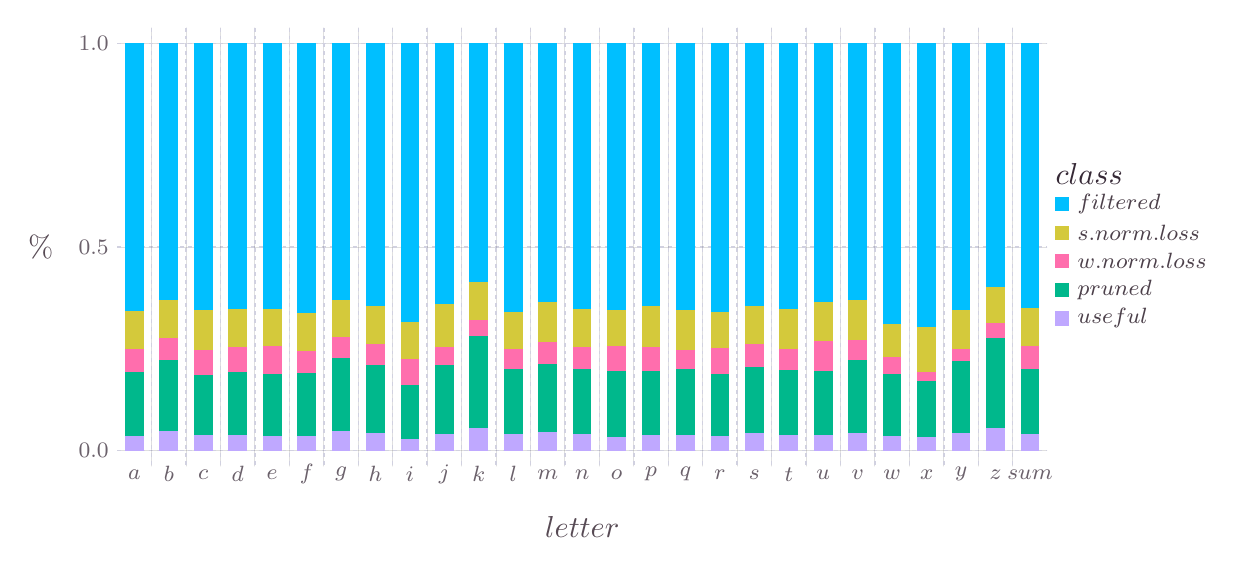
\begin{tikzpicture}[x=1mm,y=-1mm]
\definecolor{mycolorD4CA3A}{rgb}{0.83,0.79,0.23}
\definecolor{mycolor4C404B}{rgb}{0.3,0.25,0.29}
\definecolor{mycolor00BFFF}{rgb}{0,0.75,1}
\definecolor{mycolorD0D0E0}{rgb}{0.82,0.82,0.88}
\definecolor{mycolor362A35}{rgb}{0.21,0.16,0.21}
\definecolor{mycolor000000}{rgb}{0,0,0}
\definecolor{mycolor000000}{rgb}{0,0,0}
\definecolor{mycolor00B78D}{rgb}{0,0.72,0.55}
\definecolor{mycolor6C606B}{rgb}{0.42,0.38,0.42}
\definecolor{mycolorBEA9FF}{rgb}{0.75,0.66,1}
\definecolor{mycolorFF6DAE}{rgb}{1,0.43,0.68}
\definecolor{mycolor564A55}{rgb}{0.34,0.29,0.33}
\begin{scope}
\begin{scope}
\draw (77.07,68.39) node [text=mycolor564A55,draw=mycolor000000,draw opacity=0,rotate around={-0: (0,1.81)},inner sep=0.0]{\fontsize{3.88mm}{4.66mm}\selectfont $\text{letter}$};
\end{scope}
\begin{scope}
\draw (20.2,61.72) node [text=mycolor6C606B,rotate around={-0: (56.87,1.34)},inner sep=0.0]{\fontsize{2.82mm}{3.39mm}\selectfont $\text{a}$};
\draw (24.58,61.72) node [text=mycolor6C606B,rotate around={-0: (52.49,1.34)},inner sep=0.0]{\fontsize{2.82mm}{3.39mm}\selectfont $\text{b}$};
\draw (28.95,61.72) node [text=mycolor6C606B,rotate around={-0: (48.12,1.34)},inner sep=0.0]{\fontsize{2.82mm}{3.39mm}\selectfont $\text{c}$};
\draw (33.33,61.72) node [text=mycolor6C606B,rotate around={-0: (43.74,1.34)},inner sep=0.0]{\fontsize{2.82mm}{3.39mm}\selectfont $\text{d}$};
\draw (37.7,61.72) node [text=mycolor6C606B,rotate around={-0: (39.37,1.34)},inner sep=0.0]{\fontsize{2.82mm}{3.39mm}\selectfont $\text{e}$};
\draw (42.08,61.72) node [text=mycolor6C606B,rotate around={-0: (35,1.34)},inner sep=0.0]{\fontsize{2.82mm}{3.39mm}\selectfont $\text{f}$};
\draw (46.45,61.72) node [text=mycolor6C606B,rotate around={-0: (30.62,1.34)},inner sep=0.0]{\fontsize{2.82mm}{3.39mm}\selectfont $\text{g}$};
\draw (50.83,61.72) node [text=mycolor6C606B,rotate around={-0: (26.25,1.34)},inner sep=0.0]{\fontsize{2.82mm}{3.39mm}\selectfont $\text{h}$};
\draw (55.2,61.72) node [text=mycolor6C606B,rotate around={-0: (21.87,1.34)},inner sep=0.0]{\fontsize{2.82mm}{3.39mm}\selectfont $\text{i}$};
\draw (59.57,61.72) node [text=mycolor6C606B,rotate around={-0: (17.5,1.34)},inner sep=0.0]{\fontsize{2.82mm}{3.39mm}\selectfont $\text{j}$};
\draw (63.95,61.72) node [text=mycolor6C606B,rotate around={-0: (13.12,1.34)},inner sep=0.0]{\fontsize{2.82mm}{3.39mm}\selectfont $\text{k}$};
\draw (68.32,61.72) node [text=mycolor6C606B,rotate around={-0: (8.75,1.34)},inner sep=0.0]{\fontsize{2.82mm}{3.39mm}\selectfont $\text{l}$};
\draw (72.7,61.72) node [text=mycolor6C606B,rotate around={-0: (4.37,1.34)},inner sep=0.0]{\fontsize{2.82mm}{3.39mm}\selectfont $\text{m}$};
\draw (77.07,61.72) node [text=mycolor6C606B,rotate around={-0: (0,1.34)},inner sep=0.0]{\fontsize{2.82mm}{3.39mm}\selectfont $\text{n}$};
\draw (81.45,61.72) node [text=mycolor6C606B,rotate around={-0: (-4.37,1.34)},inner sep=0.0]{\fontsize{2.82mm}{3.39mm}\selectfont $\text{o}$};
\draw (85.82,61.72) node [text=mycolor6C606B,rotate around={-0: (-8.75,1.34)},inner sep=0.0]{\fontsize{2.82mm}{3.39mm}\selectfont $\text{p}$};
\draw (90.2,61.72) node [text=mycolor6C606B,rotate around={-0: (-13.12,1.34)},inner sep=0.0]{\fontsize{2.82mm}{3.39mm}\selectfont $\text{q}$};
\draw (94.57,61.72) node [text=mycolor6C606B,rotate around={-0: (-17.5,1.34)},inner sep=0.0]{\fontsize{2.82mm}{3.39mm}\selectfont $\text{r}$};
\draw (98.94,61.72) node [text=mycolor6C606B,rotate around={-0: (-21.87,1.34)},inner sep=0.0]{\fontsize{2.82mm}{3.39mm}\selectfont $\text{s}$};
\draw (103.32,61.72) node [text=mycolor6C606B,rotate around={-0: (-26.25,1.34)},inner sep=0.0]{\fontsize{2.82mm}{3.39mm}\selectfont $\text{t}$};
\draw (107.69,61.72) node [text=mycolor6C606B,rotate around={-0: (-30.62,1.34)},inner sep=0.0]{\fontsize{2.82mm}{3.39mm}\selectfont $\text{u}$};
\draw (112.07,61.72) node [text=mycolor6C606B,rotate around={-0: (-35,1.34)},inner sep=0.0]{\fontsize{2.82mm}{3.39mm}\selectfont $\text{v}$};
\draw (116.44,61.72) node [text=mycolor6C606B,rotate around={-0: (-39.37,1.34)},inner sep=0.0]{\fontsize{2.82mm}{3.39mm}\selectfont $\text{w}$};
\draw (120.82,61.72) node [text=mycolor6C606B,rotate around={-0: (-43.74,1.34)},inner sep=0.0]{\fontsize{2.82mm}{3.39mm}\selectfont $\text{x}$};
\draw (125.19,61.72) node [text=mycolor6C606B,rotate around={-0: (-48.12,1.34)},inner sep=0.0]{\fontsize{2.82mm}{3.39mm}\selectfont $\text{y}$};
\draw (129.57,61.72) node [text=mycolor6C606B,rotate around={-0: (-52.49,1.34)},inner sep=0.0]{\fontsize{2.82mm}{3.39mm}\selectfont $\text{z}$};
\draw (133.94,61.72) node [text=mycolor6C606B,rotate around={-0: (-56.87,1.34)},inner sep=0.0]{\fontsize{2.82mm}{3.39mm}\selectfont $\text{sum}$};
\end{scope}
\begin{scope}
\begin{scope}
\draw (139.94,27.42) node [text=mycolor4C404B,rotate around={-0: (5.62,5.44)},right,inner sep=0.0]{\fontsize{2.82mm}{3.39mm}\selectfont $\text{filtered}$};
\draw (139.94,31.04) node [text=mycolor4C404B,rotate around={-0: (5.62,1.81)},right,inner sep=0.0]{\fontsize{2.82mm}{3.39mm}\selectfont $\text{s.norm. loss}$};
\draw (139.94,34.67) node [text=mycolor4C404B,rotate around={-0: (5.62,-1.81)},right,inner sep=0.0]{\fontsize{2.82mm}{3.39mm}\selectfont $\text{w.norm. loss}$};
\draw (139.94,38.3) node [text=mycolor4C404B,rotate around={-0: (5.62,-5.44)},right,inner sep=0.0]{\fontsize{2.82mm}{3.39mm}\selectfont $\text{pruned}$};
\draw (139.94,41.92) node [text=mycolor4C404B,rotate around={-0: (5.62,-9.07)},right,inner sep=0.0]{\fontsize{2.82mm}{3.39mm}\selectfont $\text{useful}$};
\end{scope}
\begin{scope}
\path [fill=mycolor00BFFF,draw=mycolor000000,draw opacity=0] (137.13,26.51) rectangle +(1.81,1.81);
\path [fill=mycolorD4CA3A,draw=mycolor000000,draw opacity=0] (137.13,30.14) rectangle +(1.81,1.81);
\path [fill=mycolorFF6DAE,draw=mycolor000000,draw opacity=0] (137.13,33.76) rectangle +(1.81,1.81);
\path [fill=mycolor00B78D,draw=mycolor000000,draw opacity=0] (137.13,37.39) rectangle +(1.81,1.81);
\path [fill=mycolorBEA9FF,draw=mycolor000000,draw opacity=0] (137.13,41.02) rectangle +(1.81,1.81);
\end{scope}
\begin{scope}
\draw (137.13,23.6) node [text=mycolor362A35,draw=mycolor000000,draw opacity=0,rotate around={-0: (9.44,0.19)},right,inner sep=0.0]{\fontsize{3.88mm}{4.66mm}\selectfont $\text{class}$};
\end{scope}
\end{scope}
\begin{scope}
\clip  (18.02,5) -- (136.13,5) -- (136.13,60.72) -- (18.02,60.72);
\begin{scope}
\clip  (18.02,5) -- (136.13,5) -- (136.13,60.72) -- (18.02,60.72);
\path [fill=mycolor000000,fill opacity=0,draw=mycolor000000,draw opacity=0] (18.02,5) rectangle +(118.11,55.72);
\end{scope}
\begin{scope}
[dash pattern=on 0.5mm off 0.5mm,line width=0.2mm]
\path [fill=mycolor000000,draw=mycolorD0D0E0]  (18.02,58.72) -- (136.13,58.72);
\path [fill=mycolor000000,draw=mycolorD0D0E0]  (18.02,32.86) -- (136.13,32.86);
\path [fill=mycolor000000,draw=mycolorD0D0E0]  (18.02,7) -- (136.13,7);
\end{scope}
\begin{scope}
[dash pattern=on 0.5mm off 0.5mm,line width=0.2mm]
\path [fill=mycolor000000,draw=mycolorD0D0E0]  (22.39,5) -- (22.39,60.72);
\path [fill=mycolor000000,draw=mycolorD0D0E0]  (26.77,5) -- (26.77,60.72);
\path [fill=mycolor000000,draw=mycolorD0D0E0]  (31.14,5) -- (31.14,60.72);
\path [fill=mycolor000000,draw=mycolorD0D0E0]  (35.52,5) -- (35.52,60.72);
\path [fill=mycolor000000,draw=mycolorD0D0E0]  (39.89,5) -- (39.89,60.72);
\path [fill=mycolor000000,draw=mycolorD0D0E0]  (44.26,5) -- (44.26,60.72);
\path [fill=mycolor000000,draw=mycolorD0D0E0]  (48.64,5) -- (48.64,60.72);
\path [fill=mycolor000000,draw=mycolorD0D0E0]  (53.01,5) -- (53.01,60.72);
\path [fill=mycolor000000,draw=mycolorD0D0E0]  (57.39,5) -- (57.39,60.72);
\path [fill=mycolor000000,draw=mycolorD0D0E0]  (61.76,5) -- (61.76,60.72);
\path [fill=mycolor000000,draw=mycolorD0D0E0]  (66.14,5) -- (66.14,60.72);
\path [fill=mycolor000000,draw=mycolorD0D0E0]  (70.51,5) -- (70.51,60.72);
\path [fill=mycolor000000,draw=mycolorD0D0E0]  (74.88,5) -- (74.88,60.72);
\path [fill=mycolor000000,draw=mycolorD0D0E0]  (79.26,5) -- (79.26,60.72);
\path [fill=mycolor000000,draw=mycolorD0D0E0]  (83.63,5) -- (83.63,60.72);
\path [fill=mycolor000000,draw=mycolorD0D0E0]  (88.01,5) -- (88.01,60.72);
\path [fill=mycolor000000,draw=mycolorD0D0E0]  (92.38,5) -- (92.38,60.72);
\path [fill=mycolor000000,draw=mycolorD0D0E0]  (96.76,5) -- (96.76,60.72);
\path [fill=mycolor000000,draw=mycolorD0D0E0]  (101.13,5) -- (101.13,60.72);
\path [fill=mycolor000000,draw=mycolorD0D0E0]  (105.51,5) -- (105.51,60.72);
\path [fill=mycolor000000,draw=mycolorD0D0E0]  (109.88,5) -- (109.88,60.72);
\path [fill=mycolor000000,draw=mycolorD0D0E0]  (114.25,5) -- (114.25,60.72);
\path [fill=mycolor000000,draw=mycolorD0D0E0]  (118.63,5) -- (118.63,60.72);
\path [fill=mycolor000000,draw=mycolorD0D0E0]  (123,5) -- (123,60.72);
\path [fill=mycolor000000,draw=mycolorD0D0E0]  (127.38,5) -- (127.38,60.72);
\path [fill=mycolor000000,draw=mycolorD0D0E0]  (131.75,5) -- (131.75,60.72);
\end{scope}
\begin{scope}
\begin{scope}
[line width=0.3mm]
\begin{scope}
\path [fill=mycolorBEA9FF,draw=mycolor000000,draw opacity=0] (19.02,56.82) rectangle +(2.37,1.89);
\path [fill=mycolorBEA9FF,draw=mycolor000000,draw opacity=0] (23.39,56.26) rectangle +(2.37,2.46);
\path [fill=mycolorBEA9FF,draw=mycolor000000,draw opacity=0] (27.77,56.73) rectangle +(2.37,1.99);
\path [fill=mycolorBEA9FF,draw=mycolor000000,draw opacity=0] (32.14,56.7) rectangle +(2.37,2.01);
\path [fill=mycolorBEA9FF,draw=mycolor000000,draw opacity=0] (36.52,56.87) rectangle +(2.37,1.84);
\path [fill=mycolorBEA9FF,draw=mycolor000000,draw opacity=0] (40.89,56.81) rectangle +(2.37,1.9);
\path [fill=mycolorBEA9FF,draw=mycolor000000,draw opacity=0] (45.26,56.26) rectangle +(2.37,2.46);
\path [fill=mycolorBEA9FF,draw=mycolor000000,draw opacity=0] (49.64,56.46) rectangle +(2.37,2.26);
\path [fill=mycolorBEA9FF,draw=mycolor000000,draw opacity=0] (54.01,57.27) rectangle +(2.37,1.45);
\path [fill=mycolorBEA9FF,draw=mycolor000000,draw opacity=0] (58.39,56.61) rectangle +(2.37,2.1);
\path [fill=mycolorBEA9FF,draw=mycolor000000,draw opacity=0] (62.76,55.79) rectangle +(2.37,2.92);
\path [fill=mycolorBEA9FF,draw=mycolor000000,draw opacity=0] (67.14,56.62) rectangle +(2.37,2.09);
\path [fill=mycolorBEA9FF,draw=mycolor000000,draw opacity=0] (71.51,56.36) rectangle +(2.37,2.36);
\path [fill=mycolorBEA9FF,draw=mycolor000000,draw opacity=0] (75.88,56.56) rectangle +(2.37,2.16);
\path [fill=mycolorBEA9FF,draw=mycolor000000,draw opacity=0] (80.26,56.98) rectangle +(2.37,1.74);
\path [fill=mycolorBEA9FF,draw=mycolor000000,draw opacity=0] (84.63,56.69) rectangle +(2.37,2.03);
\path [fill=mycolorBEA9FF,draw=mycolor000000,draw opacity=0] (89.01,56.74) rectangle +(2.37,1.97);
\path [fill=mycolorBEA9FF,draw=mycolor000000,draw opacity=0] (93.38,56.8) rectangle +(2.37,1.91);
\path [fill=mycolorBEA9FF,draw=mycolor000000,draw opacity=0] (97.76,56.52) rectangle +(2.37,2.19);
\path [fill=mycolorBEA9FF,draw=mycolor000000,draw opacity=0] (102.13,56.73) rectangle +(2.37,1.98);
\path [fill=mycolorBEA9FF,draw=mycolor000000,draw opacity=0] (106.51,56.73) rectangle +(2.37,1.99);
\path [fill=mycolorBEA9FF,draw=mycolor000000,draw opacity=0] (110.88,56.52) rectangle +(2.37,2.19);
\path [fill=mycolorBEA9FF,draw=mycolor000000,draw opacity=0] (115.25,56.8) rectangle +(2.37,1.91);
\path [fill=mycolorBEA9FF,draw=mycolor000000,draw opacity=0] (119.63,56.98) rectangle +(2.37,1.74);
\path [fill=mycolorBEA9FF,draw=mycolor000000,draw opacity=0] (124,56.46) rectangle +(2.37,2.26);
\path [fill=mycolorBEA9FF,draw=mycolor000000,draw opacity=0] (128.38,55.85) rectangle +(2.37,2.86);
\path [fill=mycolorBEA9FF,draw=mycolor000000,draw opacity=0] (132.75,56.64) rectangle +(2.37,2.08);
\path [fill=mycolor00B78D,draw=mycolor000000,draw opacity=0] (19.02,48.78) rectangle +(2.37,8.04);
\path [fill=mycolor00B78D,draw=mycolor000000,draw opacity=0] (23.39,47.19) rectangle +(2.37,9.07);
\path [fill=mycolor00B78D,draw=mycolor000000,draw opacity=0] (27.77,49.08) rectangle +(2.37,7.65);
\path [fill=mycolor00B78D,draw=mycolor000000,draw opacity=0] (32.14,48.78) rectangle +(2.37,7.92);
\path [fill=mycolor00B78D,draw=mycolor000000,draw opacity=0] (36.52,49) rectangle +(2.37,7.87);
\path [fill=mycolor00B78D,draw=mycolor000000,draw opacity=0] (40.89,48.87) rectangle +(2.37,7.94);
\path [fill=mycolor00B78D,draw=mycolor000000,draw opacity=0] (45.26,47.01) rectangle +(2.37,9.24);
\path [fill=mycolor00B78D,draw=mycolor000000,draw opacity=0] (49.64,47.86) rectangle +(2.37,8.6);
\path [fill=mycolor00B78D,draw=mycolor000000,draw opacity=0] (54.01,50.39) rectangle +(2.37,6.88);
\path [fill=mycolor00B78D,draw=mycolor000000,draw opacity=0] (58.39,47.85) rectangle +(2.37,8.77);
\path [fill=mycolor00B78D,draw=mycolor000000,draw opacity=0] (62.76,44.21) rectangle +(2.37,11.58);
\path [fill=mycolor00B78D,draw=mycolor000000,draw opacity=0] (67.14,48.41) rectangle +(2.37,8.21);
\path [fill=mycolor00B78D,draw=mycolor000000,draw opacity=0] (71.51,47.73) rectangle +(2.37,8.63);
\path [fill=mycolor00B78D,draw=mycolor000000,draw opacity=0] (75.88,48.35) rectangle +(2.37,8.21);
\path [fill=mycolor00B78D,draw=mycolor000000,draw opacity=0] (80.26,48.64) rectangle +(2.37,8.34);
\path [fill=mycolor00B78D,draw=mycolor000000,draw opacity=0] (84.63,48.58) rectangle +(2.37,8.11);
\path [fill=mycolor00B78D,draw=mycolor000000,draw opacity=0] (89.01,48.33) rectangle +(2.37,8.41);
\path [fill=mycolor00B78D,draw=mycolor000000,draw opacity=0] (93.38,48.97) rectangle +(2.37,7.83);
\path [fill=mycolor00B78D,draw=mycolor000000,draw opacity=0] (97.76,48.04) rectangle +(2.37,8.48);
\path [fill=mycolor00B78D,draw=mycolor000000,draw opacity=0] (102.13,48.45) rectangle +(2.37,8.28);
\path [fill=mycolor00B78D,draw=mycolor000000,draw opacity=0] (106.51,48.64) rectangle +(2.37,8.09);
\path [fill=mycolor00B78D,draw=mycolor000000,draw opacity=0] (110.88,47.21) rectangle +(2.37,9.31);
\path [fill=mycolor00B78D,draw=mycolor000000,draw opacity=0] (115.25,48.95) rectangle +(2.37,7.86);
\path [fill=mycolor00B78D,draw=mycolor000000,draw opacity=0] (119.63,49.81) rectangle +(2.37,7.17);
\path [fill=mycolor00B78D,draw=mycolor000000,draw opacity=0] (124,47.36) rectangle +(2.37,9.1);
\path [fill=mycolor00B78D,draw=mycolor000000,draw opacity=0] (128.38,44.35) rectangle +(2.37,11.5);
\path [fill=mycolor00B78D,draw=mycolor000000,draw opacity=0] (132.75,48.31) rectangle +(2.37,8.33);
\path [fill=mycolorFF6DAE,draw=mycolor000000,draw opacity=0] (19.02,45.75) rectangle +(2.37,3.03);
\path [fill=mycolorFF6DAE,draw=mycolor000000,draw opacity=0] (23.39,44.4) rectangle +(2.37,2.79);
\path [fill=mycolorFF6DAE,draw=mycolor000000,draw opacity=0] (27.77,45.98) rectangle +(2.37,3.1);
\path [fill=mycolorFF6DAE,draw=mycolor000000,draw opacity=0] (32.14,45.55) rectangle +(2.37,3.23);
\path [fill=mycolorFF6DAE,draw=mycolor000000,draw opacity=0] (36.52,45.38) rectangle +(2.37,3.62);
\path [fill=mycolorFF6DAE,draw=mycolor000000,draw opacity=0] (40.89,46) rectangle +(2.37,2.87);
\path [fill=mycolorFF6DAE,draw=mycolor000000,draw opacity=0] (45.26,44.33) rectangle +(2.37,2.68);
\path [fill=mycolorFF6DAE,draw=mycolor000000,draw opacity=0] (49.64,45.21) rectangle +(2.37,2.64);
\path [fill=mycolorFF6DAE,draw=mycolor000000,draw opacity=0] (54.01,47.04) rectangle +(2.37,3.35);
\path [fill=mycolorFF6DAE,draw=mycolor000000,draw opacity=0] (58.39,45.57) rectangle +(2.37,2.28);
\path [fill=mycolorFF6DAE,draw=mycolor000000,draw opacity=0] (62.76,42.07) rectangle +(2.37,2.14);
\path [fill=mycolorFF6DAE,draw=mycolor000000,draw opacity=0] (67.14,45.85) rectangle +(2.37,2.56);
\path [fill=mycolorFF6DAE,draw=mycolor000000,draw opacity=0] (71.51,44.96) rectangle +(2.37,2.77);
\path [fill=mycolorFF6DAE,draw=mycolor000000,draw opacity=0] (75.88,45.56) rectangle +(2.37,2.78);
\path [fill=mycolorFF6DAE,draw=mycolor000000,draw opacity=0] (80.26,45.38) rectangle +(2.37,3.25);
\path [fill=mycolorFF6DAE,draw=mycolor000000,draw opacity=0] (84.63,45.51) rectangle +(2.37,3.07);
\path [fill=mycolorFF6DAE,draw=mycolor000000,draw opacity=0] (89.01,45.9) rectangle +(2.37,2.43);
\path [fill=mycolorFF6DAE,draw=mycolor000000,draw opacity=0] (93.38,45.65) rectangle +(2.37,3.32);
\path [fill=mycolorFF6DAE,draw=mycolor000000,draw opacity=0] (97.76,45.22) rectangle +(2.37,2.82);
\path [fill=mycolorFF6DAE,draw=mycolor000000,draw opacity=0] (102.13,45.83) rectangle +(2.37,2.63);
\path [fill=mycolorFF6DAE,draw=mycolor000000,draw opacity=0] (106.51,44.75) rectangle +(2.37,3.89);
\path [fill=mycolorFF6DAE,draw=mycolor000000,draw opacity=0] (110.88,44.63) rectangle +(2.37,2.58);
\path [fill=mycolorFF6DAE,draw=mycolor000000,draw opacity=0] (115.25,46.83) rectangle +(2.37,2.12);
\path [fill=mycolorFF6DAE,draw=mycolor000000,draw opacity=0] (119.63,48.69) rectangle +(2.37,1.12);
\path [fill=mycolorFF6DAE,draw=mycolor000000,draw opacity=0] (124,45.79) rectangle +(2.37,1.56);
\path [fill=mycolorFF6DAE,draw=mycolor000000,draw opacity=0] (128.38,42.47) rectangle +(2.37,1.88);
\path [fill=mycolorFF6DAE,draw=mycolor000000,draw opacity=0] (132.75,45.41) rectangle +(2.37,2.9);
\path [fill=mycolorD4CA3A,draw=mycolor000000,draw opacity=0] (19.02,40.99) rectangle +(2.37,4.76);
\path [fill=mycolorD4CA3A,draw=mycolor000000,draw opacity=0] (23.39,39.56) rectangle +(2.37,4.84);
\path [fill=mycolorD4CA3A,draw=mycolor000000,draw opacity=0] (27.77,40.91) rectangle +(2.37,5.07);
\path [fill=mycolorD4CA3A,draw=mycolor000000,draw opacity=0] (32.14,40.7) rectangle +(2.37,4.85);
\path [fill=mycolorD4CA3A,draw=mycolor000000,draw opacity=0] (36.52,40.71) rectangle +(2.37,4.68);
\path [fill=mycolorD4CA3A,draw=mycolor000000,draw opacity=0] (40.89,41.2) rectangle +(2.37,4.81);
\path [fill=mycolorD4CA3A,draw=mycolor000000,draw opacity=0] (45.26,39.54) rectangle +(2.37,4.79);
\path [fill=mycolorD4CA3A,draw=mycolor000000,draw opacity=0] (49.64,40.34) rectangle +(2.37,4.87);
\path [fill=mycolorD4CA3A,draw=mycolor000000,draw opacity=0] (54.01,42.33) rectangle +(2.37,4.71);
\path [fill=mycolorD4CA3A,draw=mycolor000000,draw opacity=0] (58.39,40.11) rectangle +(2.37,5.46);
\path [fill=mycolorD4CA3A,draw=mycolor000000,draw opacity=0] (62.76,37.27) rectangle +(2.37,4.8);
\path [fill=mycolorD4CA3A,draw=mycolor000000,draw opacity=0] (67.14,41.06) rectangle +(2.37,4.79);
\path [fill=mycolorD4CA3A,draw=mycolor000000,draw opacity=0] (71.51,39.88) rectangle +(2.37,5.08);
\path [fill=mycolorD4CA3A,draw=mycolor000000,draw opacity=0] (75.88,40.7) rectangle +(2.37,4.86);
\path [fill=mycolorD4CA3A,draw=mycolor000000,draw opacity=0] (80.26,40.81) rectangle +(2.37,4.57);
\path [fill=mycolorD4CA3A,draw=mycolor000000,draw opacity=0] (84.63,40.41) rectangle +(2.37,5.1);
\path [fill=mycolorD4CA3A,draw=mycolor000000,draw opacity=0] (89.01,40.88) rectangle +(2.37,5.02);
\path [fill=mycolorD4CA3A,draw=mycolor000000,draw opacity=0] (93.38,41.05) rectangle +(2.37,4.6);
\path [fill=mycolorD4CA3A,draw=mycolor000000,draw opacity=0] (97.76,40.3) rectangle +(2.37,4.92);
\path [fill=mycolorD4CA3A,draw=mycolor000000,draw opacity=0] (102.13,40.73) rectangle +(2.37,5.1);
\path [fill=mycolorD4CA3A,draw=mycolor000000,draw opacity=0] (106.51,39.82) rectangle +(2.37,4.92);
\path [fill=mycolorD4CA3A,draw=mycolor000000,draw opacity=0] (110.88,39.64) rectangle +(2.37,4.99);
\path [fill=mycolorD4CA3A,draw=mycolor000000,draw opacity=0] (115.25,42.61) rectangle +(2.37,4.22);
\path [fill=mycolorD4CA3A,draw=mycolor000000,draw opacity=0] (119.63,43) rectangle +(2.37,5.69);
\path [fill=mycolorD4CA3A,draw=mycolor000000,draw opacity=0] (124,40.89) rectangle +(2.37,4.9);
\path [fill=mycolorD4CA3A,draw=mycolor000000,draw opacity=0] (128.38,37.95) rectangle +(2.37,4.51);
\path [fill=mycolorD4CA3A,draw=mycolor000000,draw opacity=0] (132.75,40.54) rectangle +(2.37,4.87);
\path [fill=mycolor00BFFF,draw=mycolor000000,draw opacity=0] (19.02,7) rectangle +(2.37,33.99);
\path [fill=mycolor00BFFF,draw=mycolor000000,draw opacity=0] (23.39,7) rectangle +(2.37,32.56);
\path [fill=mycolor00BFFF,draw=mycolor000000,draw opacity=0] (27.77,7) rectangle +(2.37,33.91);
\path [fill=mycolor00BFFF,draw=mycolor000000,draw opacity=0] (32.14,7) rectangle +(2.37,33.7);
\path [fill=mycolor00BFFF,draw=mycolor000000,draw opacity=0] (36.52,7) rectangle +(2.37,33.71);
\path [fill=mycolor00BFFF,draw=mycolor000000,draw opacity=0] (40.89,7) rectangle +(2.37,34.2);
\path [fill=mycolor00BFFF,draw=mycolor000000,draw opacity=0] (45.26,7) rectangle +(2.37,32.54);
\path [fill=mycolor00BFFF,draw=mycolor000000,draw opacity=0] (49.64,7) rectangle +(2.37,33.34);
\path [fill=mycolor00BFFF,draw=mycolor000000,draw opacity=0] (54.01,7) rectangle +(2.37,35.33);
\path [fill=mycolor00BFFF,draw=mycolor000000,draw opacity=0] (58.39,7) rectangle +(2.37,33.11);
\path [fill=mycolor00BFFF,draw=mycolor000000,draw opacity=0] (62.76,7) rectangle +(2.37,30.27);
\path [fill=mycolor00BFFF,draw=mycolor000000,draw opacity=0] (67.14,7) rectangle +(2.37,34.06);
\path [fill=mycolor00BFFF,draw=mycolor000000,draw opacity=0] (71.51,7) rectangle +(2.37,32.88);
\path [fill=mycolor00BFFF,draw=mycolor000000,draw opacity=0] (75.88,7) rectangle +(2.37,33.7);
\path [fill=mycolor00BFFF,draw=mycolor000000,draw opacity=0] (80.26,7) rectangle +(2.37,33.81);
\path [fill=mycolor00BFFF,draw=mycolor000000,draw opacity=0] (84.63,7) rectangle +(2.37,33.41);
\path [fill=mycolor00BFFF,draw=mycolor000000,draw opacity=0] (89.01,7) rectangle +(2.37,33.88);
\path [fill=mycolor00BFFF,draw=mycolor000000,draw opacity=0] (93.38,7) rectangle +(2.37,34.05);
\path [fill=mycolor00BFFF,draw=mycolor000000,draw opacity=0] (97.76,7) rectangle +(2.37,33.3);
\path [fill=mycolor00BFFF,draw=mycolor000000,draw opacity=0] (102.13,7) rectangle +(2.37,33.73);
\path [fill=mycolor00BFFF,draw=mycolor000000,draw opacity=0] (106.51,7) rectangle +(2.37,32.82);
\path [fill=mycolor00BFFF,draw=mycolor000000,draw opacity=0] (110.88,7) rectangle +(2.37,32.64);
\path [fill=mycolor00BFFF,draw=mycolor000000,draw opacity=0] (115.25,7) rectangle +(2.37,35.61);
\path [fill=mycolor00BFFF,draw=mycolor000000,draw opacity=0] (119.63,7) rectangle +(2.37,36);
\path [fill=mycolor00BFFF,draw=mycolor000000,draw opacity=0] (124,7) rectangle +(2.37,33.89);
\path [fill=mycolor00BFFF,draw=mycolor000000,draw opacity=0] (128.38,7) rectangle +(2.37,30.95);
\path [fill=mycolor00BFFF,draw=mycolor000000,draw opacity=0] (132.75,7) rectangle +(2.37,33.54);
\end{scope}
\end{scope}
\end{scope}
\end{scope}
\begin{scope}
\draw (17.02,58.72) node [text=mycolor6C606B,rotate around={-0: (-2.01,-25.86)},left,inner sep=0.0]{\fontsize{2.82mm}{3.39mm}\selectfont $\text{0.0}$};
\draw (17.02,32.86) node [text=mycolor6C606B,rotate around={-0: (-2.01,-0)},left,inner sep=0.0]{\fontsize{2.82mm}{3.39mm}\selectfont $\text{0.5}$};
\draw (17.02,7) node [text=mycolor6C606B,rotate around={-0: (-2.01,25.86)},left,inner sep=0.0]{\fontsize{2.82mm}{3.39mm}\selectfont $\text{1.0}$};
\end{scope}
\begin{scope}
\draw (10,32.86) node [text=mycolor564A55,draw=mycolor000000,draw opacity=0,rotate around={-0: (-1.5,0)},left,inner sep=0.0]{\fontsize{3.88mm}{4.66mm}\selectfont $\text{\%}$};
\end{scope}
\end{scope}
\end{tikzpicture}

    \caption{Relative amount of pruned data per letter}
    \label{fig:clean_up_sums}
\end{figure}

We perform the following clean up steps:

\begin{enumerate}
\itemsep0em
\item download and parsing
\item string filtering
\item string normalization
\item word normalization
\item pruning
\end{enumerate}

Note that swapping the string-based steps does not lead a different output. \autoref{fig:clean_up_sums} show how much data is pruned by every step. The exact numbers can be found in \autoref{tab:clean_up_numbers}.

\subsection{Download and Parsing}
\label{ssec:baseline:data:download}
As a first step we download the raw data from the Google server. A complete list of download URLs can be obtained here:

\url{https://storage.googleapis.com/books/ngrams/books/datasetsv2.html}

The data is mangled by a high-performance C++ implementation to speed-up the upcoming steps. During the first steps, only the nGram content is required without any knowledge of the actual time series data. We exploit this fact and delay the actual parsing and storage of the time series until the data is required and focus on the handling of the string data as long as possible.

\subsection{String filtering}
\label{ssec:baseline:data:filter}
It seems that the nGrams that Google extracted does not only contain pure words but also punctuation characters and word classes. To simplify storage of the strings and because our users are not interested in searching for whole word types, we filter out all entries that contain characters of the following class:

\code{\[_.,!'0-9\]}

\subsection{String Normalization}
\label{ssec:baseline:data:snorm}
Since the data the nGrams are described by Unicode strings, there may exist string describing the same content. We apply NFKC normalization as described in \cite{unicode8annex15} to solve this issue. Furthermore we lowercase all inputs with respect to the Unicode standard. If this procedure will lead to duplicate nGrams, they are joined by adding the coresponding time series data.

Notice that the lowercase transformation may not work as expected for other languages than English since it may lead to a lose of important information.

\subsection{Word Normalization}
\label{ssec:baseline:data:wnorm}
The words forming the nGrams exist in multiple variants, e.g. different terms for verbs or singular and plural form for nouns. Naturally the resulting time series are very similar and do not contain valuable information, neither for our algorithms nor for a human analyst. We solve this issue by applying the WordNet lemmatizer (\cite{wordnet}) and afterwards the snowball stemmer (\cite{porter2}) to all words. In case of same output nGrams the related time series are added again.

As for the former transformation step be aware of the language problem. Other languages may require other word normalization techniques. Also there may be more advanced techniques that exploit the knowledge of the entire nGram instead of single words.

We decided not to run any OCR (optical character recognization) error recognization since we are not aware of any general purpose approach that does not transform rare words or names like a na\"{\i}ve spell checker would do.

\subsection{Pruning}
\label{ssec:baseline:data:prune}
The original data sets contains a lot of very rare nGrams that, in our opinion, do not provide enough statistical information to be considered during the further analysis. The same applies to all nGrams for the early years that are contained in the data. We decided to only use the last \num{256} years of the time series data and that we drop all nGrams where the related match count time series is too small, or in mathematical terms where $\sum_{1753 \leq y \leq 2008} v_{0, y} < 1000$ ($v_0$ is the "match count") applies. Notice that this is the first step where the actual time series content is required. Therefore it is also the first step where we parse the time series data for all nGram strings which survived up to this point.

The selection of the time range of \num{256} years has other advantages apart from the pure pruning. Since it is a power of \num{2} it is easier to apply many transformations (e.g. Fourier or Discrete Wavelet Transformation) to it without the need to think about and justify additional edge case handling.

\chapter{Algorithm}
\label{ch:algorithm}

\dots



\section{Discrete Wavelet Transform}
\label{sec:algorithm:wavelet}

\begin{figure}
    \centering
    \begin{tikzpicture}[
        arrow/.style={
            ->,
            >=stealth
        },
        node/.style={
            draw,
            fill=white,
            font=\scriptsize
        },
        tnode/.style={
            node,
            minimum width=1.25cm,
            minimum height=0.75cm,
            rectangle
        },
        rnode/.style={
            node,
            minimum width=0.75cm,
            minimum height=0.75cm,
            circle
        },
        xabove/.style args={of #1}{above=0.5cm of #1.north}
    ]

    \begin{axis}[
        xlabel={x},
        ylabel={y},
        fullwidth,
        height=0.30\textwidth
    ]
        \addplot [mark=*,color=kit-blue] table {
            1 -1
            2  1
            3  0.5
            4  1.5
            5  4
            6  2
            7  2
            8 -2
        };

        \node (a1) at (1, -1) {};
        \node (a2) at (2,  1) {};
        \node (a3) at (3,  0.5) {};
        \node (a4) at (4,  1.5) {};
        \node (a5) at (5,  4) {};
        \node (a6) at (6,  2) {};
        \node (a7) at (7,  2) {};
        \node (a8) at (8, -2) {};
    \end{axis}

    \node (f12) [fit=(a1)(a2)] {};
    \node (f34) [fit=(a3)(a4)] {};
    \node (f56) [fit=(a5)(a6)] {};
    \node (f78) [fit=(a7)(a8)] {};

    \node (n12) [tnode,xabove=of f12] {$-1 \cdot \sqrt{2}$};  % =0
    \node (n34) [tnode,xabove=of f34] {$-0.5 \cdot \sqrt{2}$};  % =1
    \node (n56) [tnode,xabove=of f56] {$1 \cdot \sqrt{2}$};  % =3
    \node (n78) [tnode,xabove=of f78] {$2 \cdot \sqrt{2}$};  % =0

    \node (f1234) [fit=(n12)(n34)] {};
    \node (f5678) [fit=(n56)(n78)] {};

    \node (n1234) [tnode,xabove=of f1234] {$-0.5 \cdot \sqrt{4}$}; % =0.5
    \node (n5678) [tnode,xabove=of f5678] {$1.5 \cdot \sqrt{4}$}; % =1.5

    \node (f12345678) [fit=(n1234)(n5678)] {};

    \node (n12345678) [tnode,xabove=of f12345678] {$-0.5 \cdot \sqrt{8}$}; % =1

    \node (root) [rnode,above=1cm of n12345678] {$1 \cdot \sqrt{8}$};

    \draw[arrow,dashed] (n12.south) -- (a1);
    \draw[arrow,dashed] (n12.south) -- (a2);
    \draw[arrow,dashed] (n34.south) -- (a3);
    \draw[arrow,dashed] (n34.south) -- (a4);
    \draw[arrow,dashed] (n56.south) -- (a5);
    \draw[arrow,dashed] (n56.south) -- (a6);
    \draw[arrow,dashed] (n78.south) -- (a7);
    \draw[arrow,dashed] (n78.south) -- (a8);

    \draw[arrow] (n1234.south) -- (n12.north);
    \draw[arrow] (n1234.south) -- (n34.north);
    \draw[arrow] (n5678.south) -- (n56.north);
    \draw[arrow] (n5678.south) -- (n78.north);

    \draw[arrow] (n12345678.south) -- (n1234.north);
    \draw[arrow] (n12345678.south) -- (n5678.north);

    \draw[arrow] (root.south) -- (n12345678.north);
\end{tikzpicture}

    \caption{Wavelet Tree Construction}
    \label{fig:wavelet_tree_example}
\end{figure}

First of all, we need to find a time series representation that enables us to compare different series on different time scales and different granularities. While the granularity requirement is met by a Fourier Transform, it is not sufficient for different time ranges. The reason for it is that the entire series is disassembled into frequencies that span the hole range. That makes it difficult to compare sub-ranges. So we chose a different transformation -- the Discrete Wavelet Transform under usage of the Haar Wavelet (\cite{Haar}). A special property of this kind of transform is that it deconstructs a time series into a tree-like structure as shown in \autoref{fig:wavelet_tree_example}. Note that we only support time series which length is a power of two. A generalization might be archived by the application of \cite{haar_tree_notwo}.

Now we want to discuss what data is actually transformed. It turns out that using the unsmoothed, but logarithmic data works the best. The reason for this are the following: the $\log(x + 1)$ transformation avoids the handling of too large values and as shown before results in a better value distribution. Now smoothing would certainly simply later compression attempts of the wavelet data, but it already prunes information. That alone is not a huge deal, but it gets problematic when we modify the wavelet data. Alterning the coefficients of the wavelet tree, e.g. by rounding, data conversion, tree pruning (see \autoref{sec:algorithm:pruning}) or tree merging (see \autoref{sec:algorithm:merge}); results in a unsmooth time series after restoring them from the wavelet data. So to use them afterwards a smoothing step is required. A pre-transform smoothing now would results in three steps of information loss while only smoothing after the information recovery makes parameters easier to tune and information loss easier to calculate.



\section{Tree Pruning}
\label{sec:algorithm:pruning}

\begin{algorithm}
    \KwData{Node $n$}
    \KwData{Error threshold $t$}
    \KwResult{Pruned Node $n$, resulting error increase}

    \Begin {
        \tcc{Check if children are pruned}
        $p_l$ $\leftarrow$ $\neg n.\textrm{child\_l} \lor n.\textrm{child\_l}.\textrm{pruned}$\;
        $p_r$ $\leftarrow$ $\neg n.\textrm{child\_r} \lor n.\textrm{child\_r}.\textrm{pruned}$\;
        $p_c$ $\leftarrow$ $p_l \land p_r$\;
        \BlankLine
        \tcc{Calculate maximum error increase}
        $i$ $\leftarrow$ $2^{d - l + 1}$\;
        $e$ $\leftarrow$ $|n.\textrm{x}| \cdot \sqrt{i}$\;
        \BlankLine
        \tcc{Prune if requirements are met}
        \eIf{$e < t \land p_c$}{
            $n.\textrm{pruned}$ $\leftarrow$ $1$\;
            $n.\textrm{x}$ $\leftarrow$ $0$\;
            \Return{e}\;
        }{
            \Return{0}\;
        }
    }

    \caption{pruneNode}
    \label{algo:pruneNode}
\end{algorithm}

\begin{algorithm}
    \KwData{Tree $T$}
    \KwData{Error threshold $t$}
    \KwResult{Pruned Tree $T$}

    \SetKwFunction{GetLayer}{getLayer}
    \SetKwFunction{PruneNode}{pruneNode}
    \SetKwFunction{Shuffle}{shuffle}
    \SetKwFunction{Sort}{sort}

    \Begin {
        \For{l=d \emph{\KwTo} 1}{
            $N$ $\leftarrow$ $\GetLayer{T, l}$\;
            $\Shuffle{N}$\;
            $\Sort{N}$\tcp*[r]{optional}
            \For{n $\in$ N}{
                $t$ $\leftarrow$ $t - \PruneNode{n}$\;
            }
        }
    }

    \caption{pruneTree}
    \label{algo:pruneTree}
\end{algorithm}

The first attempt to reduce the amount of data is an obvious but simple approach: pruning of sub-trees that do not hold important data. This does not entirly reflect the information loss approach we will use for the final algorithm, but it is a good milestone to grasp the idea. A tree node is pruned if the following conditions are met:

\begin{enumerate}
    \item both children are pruned
    \item setting its coefficient to $0$ would not increase the error above a certain threshold
\end{enumerate}

So pruning just equals the zeroing of the coefficient, but it allows us to remove the node entirely and save storage space since it does not contain any additional information than both pruned children and the coefficient that does not have an influence anymore. The question is in which order nodes should be tried to be pruned since this algorithm is greedy method and will stop immidiatly after the threshold is reached. We propose to shuffle the nodes first to avoid a bias to the begin or end of the time series and then to sort the shuffled nodes starting the smallest coefficient. This makes it more likely to prune more nodes instead of just some with huge coefficients. Also the results are more stable as you can see while comparing \autoref{fig:ngrams_ex2_compression_unsorted} and \autoref{fig:ngrams_ex2_compression_sorted}. The algorithm is shown in \autoref{algo:pruneTree}.

\begin{figure}
    \centering
    \input{figures/ngrams_ex2_compression_unsorted.tex}
    \caption{Compression of example nGrams, without sorting/prioritizing}
    \label{fig:ngrams_ex2_compression_unsorted}
\end{figure}

\begin{figure}
    \centering
    \begin{tikzpicture}
    \begin{axis}[
        xlabel={error threshold},
        ylabel={compression rate},
        xmode=log,
        legend pos=north east,
        fullwidth
    ]
        \addplot [mark=none,color=kit-green2] table [x=x, y=y, col sep=comma, ignore chars={"}, discard if not={label}{know}] {data/ngrams_ex2_compression_sorted.csv};
        \addplot [mark=none,color=kit-cyan] table [x=x, y=y, col sep=comma, ignore chars={"}, discard if not={label}{kiss}] {data/ngrams_ex2_compression_sorted.csv};
        \addplot [mark=none,color=kit-red] table [x=x, y=y, col sep=comma, ignore chars={"}, discard if not={label}{kind}] {data/ngrams_ex2_compression_sorted.csv};
        \addplot [mark=none,color=kit-orange] table [x=x, y=y, col sep=comma, ignore chars={"}, discard if not={label}{keep}] {data/ngrams_ex2_compression_sorted.csv};
        \legend{know,kiss,kind,keep};
    \end{axis}
\end{tikzpicture}

    \caption{Compression of example nGrams, with sorting/prioritizing}
    \label{fig:ngrams_ex2_compression_sorted}
\end{figure}



\section{Tree Merging}
\label{sec:algorithm:merge}

An important thing to point out about tree pruning is that it does not exploit the fact that there are many time series which might have the same structure. The compression is purely executed on a single series. Tree merging uses a similar idea to tree pruning but with an important difference: instead of setting the coefficient to zero it will be set to a similar entry which is already present in the database (to which we come in a moment). Therefore, the subtree is not pruned but merged with another one. This can simply be done by alterning the child pointer of a tree node. The error is calculated based on the difference of the time series resulting from the new tree and the original time series. A discussion of the error metric can be found in \autoref{sec:algorithm:error}. Keep in mind to only merge nodes into others when their children are identical.

The construction of the database of known trees\footnote{To be precise: since the trees share common subtrees, they are not real trees anymore. We will continue to referr to them as trees since it is a simple and easy to understand term.} is solved as followed: the time series are added to the database in random order. One whole input tree of an entire time series is (partly) merged into the database, then the next one and so on. For the tree merging itself we changed from a strict buttom-up approach to a queue-based approach since that results in higher compression rates. The problem with the buttom-up approach is the following: it might be that there exist very similar subtrees which are cheap to merge but a strict level-ordered merging would result in prioritizing nodes next to the leaves of the tree. That is contridictary to our goal of merging as many subtrees as possible.



\section{Error Metric}
\label{sec:algorithm:error}

The choice of the error metric, while being easy in many cases, opposes some questions in our case:

\begin{itemize}
    \item How fast can a possible implementation be, not only in terms of complexity but also in terms of constant factors due to vectorization and cache layout?
    \item How good can it justify the quality of the decompressed data recovered from wavelet tree?
    \item How well does the decompressed data it work with the later smoothing, gradient calculation and DTW?
\end{itemize}

We decided to try three different metrics during the process which are described here.


\subsection{Summerized linear distance}
\label{ssec:algorithm:error:linear}

The first metric, a linear absolute distance, is one which naturally occurs when looking for something easy to implement:

\begin{equation}\label{eq:e1}
    e_1\left(t, t'\right) = \frac{1}{m} \sum_{i=1}^m \left|t_i - t'_i\right|
\end{equation}

The upper bounds can directly be calculated during the tree merging process since the influence regarding location and amplitute of certain tree nodes are know apriory. So the upper limit is simply the sum of the re-adjusted differences of the original node and the merging partner:

\begin{equation}\label{eq:e1_up}
    \bar{e}_1\left(t, t'\right) = \frac{1}{m} \sum_{m \in \mathrm{merges}(t, t')} 2^\frac{d - m_l}{2} \left|m_x - m_y\right|
\end{equation}

Here $m_l$ stands for the level of the merged node and $m_x$ and $m_y$ for the coefficient of the original node and the merge partner. Notice that all merges are included in the sum. So even when a node gets merged after both children got merged, they children are included as well.

While the implementation is rather fast because guessing of the upper limit does not require any knowledge of the actual time series difference, it is not well suited for all applications. A compression using this metric can lead to many jumps within the decompressed time series. Also the metric tends to sacrifice huge local errors for small improvements of the overall compression rate.


\subsection{Summerized quadratic distance}
\label{ssec:algorithm:error:quadratic}

A way to put higher panilties on to huge local errors is a quadratic error function:

\begin{equation}\label{eq:e2}
    e_2\left(t, t'\right) = \frac{1}{m} \sum_{i=1}^m \left(t_i - t'_i\right)^2
\end{equation}

A drawback of this function is that the calculation requires the actual distance of the original time series and the compressed one:

\begin{equation}\label{eq:e2_up}
    \bar{e}_2\left(t, t'\right) = \frac{1}{m} \sum_{i=1}^m \bar{\delta}_i(t, t')^2
\end{equation}

Here $\bar{\delta}_i(t, t')$ is the upper limit of the distance between $t$ and $t'$ at the point in time $i$. This one can be guessed using a similar method like \autoref{eq:e1_up}.

\begin{equation}\label{eq:delta_up}
    \bar{\delta}_i\left(t, t'\right) = \sum_{m \in \mathrm{merges}(t, t')} \mathbb{1}_{m \in i} \cdot 2^{-\frac{d - m_l}{2}} \left|m_x - m_y\right|
\end{equation}

where $\mathbb{1}_{m \in i}$ describes the fact that the merge $m$ does affect the point in time $i$. Notice the minus in the exponent. Since that upper limit strictly increases with at least the amount of the real delta during each merge, the error metric will reach the user-provided limit faster than expected. So we use a hybrid approach during the merging procedure: do cheap guessing until we reach the error limit and then calculate the real error and use this as a base for the following sum-up operations. The number of recalculations increases when slowly approaching the error limit but it is still way faster than calculating the real error on every merge.


\subsection{Delta Range}
\label{ssec:algorithm:error:range}

Our last metric is an application specific one which is based on the following observation: Shifting the entire time series up or down (in terms of the $y$-Axis) does not affect the gradient. Therefore this should be allowed during the compression procedure. So we use the distance between the maximum of the delta and the minimum of the delta as an error function. Keep in mind that the delta itself is signed.

\begin{equation}\label{eq:e3}
    e_3\left(t, t'\right) = \max_{i=1}^m \left|t_i - t'_i\right| - \min_{i=1}^m \left|t_i - t'_i\right|
\end{equation}

This metric has the same drawback as the one presented in \autoref{ssec:algorithm:error:quadratic} but can guessed using a similar strategy:

\begin{equation}\label{eq:e3_up}
    \bar{e}_3\left(t, t'\right) = \max_{i=1}^m \left|\bar{\delta}_i(t, t')\right| - \min_{i=1}^m \left|\bar{\delta}_i(t, t')\right|
\end{equation}



\section{Tree as Index}
\label{sec:algorithm:asindex}

\dots



\section{Optimizations}
\label{sec:algorithm:opt}

\dots



\section{Failed Improvements}
\label{sec:algorithm:fail}

A main problem of our algorithm is its greedy nature. It merges nodes always with its nearest neighbor and therefore might make decissions that result in the fact that nodes in levels near the root might not be merged because their children do not match. We tried different approaches to solve this problem but did not succeed.


\subsection{Subtree Index}
\label{ssec:algorithm:fail:stindex}

To increase the chance that the greedy algorithm chooses merges that belong to the same subtree we tried the following method:

\begin{enumerate}
    \item select multiple nearest neighbors as candidates for a merge
    \item do this for a node which belongs to the same \num{3}-subtree (or larger ones) as well
    \item check which pairs of merges belong to the same subtree and priorize them
\end{enumerate}

This requires that we are quickly able to figure out which nodes have which parents, so we introduced a subtree and superroot index to do so. Also we need to query multiple neighbors instead of just one. Alltogether that renders the entire approach inpractical and we abandond it. Also the the compression results only improved slighly and sometimes even got worse.


\subsection{FLANN}
\label{ssec:algorithm:fail:flann}

The main goal of our algorithm is to find the best matching subtree in terms of distance. To help the greedy algorithm to archive that task we tried to use FLANN (\cite{FLANN}) to merge subtrees of size \num{3} instead of single nodes. To do so we need to ensure that the coefficients stored in the tree nodes are premultiplied like the elements in \autoref{eq:e1_up}. It turns out that the huge amount of indices required renders this method impossible to implement since it is not as memory and time efficient as plain sorted arrays. The result is that the calculation never finishes. Surprisingly the partial compression results are not even better which might be due to the fact that merging entire subtrees tends to be less aggressive compared to handling single nodes.


\subsection{Random Boosting}
\label{ssec:algorithm:fail:random}

This improvement is similar to the one presented in \autoref{ssec:algorithm:fail:stindex}. We try to find better merges by observing more neighbors. This time we tried to gather a fixed amount of neighbors and select a random one with decreasing propability bound to the rank. Then we execute a complete subtree merge. This process is repeated multiple times and the best merge is kept. We also add a merge to the set where only the nearest neighbor is used to ensure that the greedy decission never is worse due to the random elements, at least as a local outcome for that specific time series. We ended up with a heavily increased calculation time and less than \SI{5}{\percent} improvements of the compression rate.


\subsection{DTW}
\label{ssec:algorithm:fail:dtw}

One of the main limitations of the current neighborhood search is that the we are only looking for nodes which correspond to the same time span. This contridicts the later usage of the data through Dynamic Time Warping. So we tried to decouble the tree structure and subtree merging from the actual time dimensions. We limited the the search for the child nodes to a time-monotonic warping and reused the implementation of the existing DTW. For the non-leaf-nodes we did not apply any constraint since the same children policy already forces merges with the correct level and correct warping. The results of this technique were not convincing since the additional degree of freedom during the merging makes it even more unlikely to hit neighbors which belong to the same subtree. So the compression rates got worse and we dropped this approach.


\subsection{Pruning}
\label{ssec:algorithm:fail:pruning}

A possible reason for suboptimal decissions during the local node merging might be that coefficients can be quite noisy and therefore expose to many possible merges which do not really differ within their value. Because only the nearest neighbor is selected for a merge, this may result in unsane results. We tried to solve this problem by introducing additional information pruning in three variants:

\begin{enumerate}
    \item before merging
    \item during merging
    \item after merging
\end{enumerate}

The pruning zeroes low significant parts of the floating point coefficients, bit by bit, so with increasing error. So the ratio of the information loss stays approxamitly constant no matter which size the coefficient has. The idea behind this is to engage the algorithm to ignore noise within the coefficient and to have less decissions to make. On the other hand this pruning also increases the error without resulting in any compression at all and is only useful for entries that will be added to the index afterwards. Sadly the increase of the error rate overweights the desired affect of helping the greedy algorithm and therefore this approach does not have a positive effect, in all three variants.

Keep in mind that this type of pruning does not decrease the memory requirements of the tree nodes since there is no fixed cutoff but rather a individual decission how much information should be kept. So to than decrease the node size by storing a shorter representation of the coefficient you would also need to store how much information got pruned which takes so much space that it eliminates its purpose. For technical reason it is also quite difficult to store nodes with sizes not fitting into hole bytes.

\chapter{Implementation}
\label{ch:implementation}

\dots



\section{A modern approach}
\label{sec:implementation:approach}

After considering multiple ways of implementing a high-performance algorithm, we decided to use \Cpp{14} as standardized in \cite{cpp14} and under partial application of the recommendations of \cite{effective_cpp} and \cite{effective_cpp2}. This gives us the ability to have fine control over memory allocations and data structures as well as the opportunity to write modern, well-structured and reusable code. In combination with a modern compiler this results in native executables which exploit a wide variety of instruction sets of current CPUs.

\begin{sidewaysfigure}
    \centering
    \begin{tikzpicture}[
        arrow/.style={
            ->,
            >=stealth
        },
        header node/.style = {
            minimum height= 1em,
            text depth    = +0pt,
            fill          = white,
            draw
        },
        header/.style = {%
            inner ysep = +1.5em,
            append after command = {
                \pgfextra{\let\TikZlastnode\tikzlastnode}
                node [header node] (header-\TikZlastnode) at (\TikZlastnode.north) {#1}
                node [fit = (\TikZlastnode)(header-\TikZlastnode)] (h-\TikZlastnode) {}
            }
        },
        node/.style={
            draw,
            font=\scriptsize,
            align=center
        },
        tool/.style={
            node,
            rectangle,
            fill=white,
            minimum width=2.0cm,
            minimum height=0.75cm
        },
        cpp/.style={
            tool,
            fill=kit-cyan!10
        },
        julia/.style={
            tool,
            fill=kit-red!10
        },
        python/.style={
            tool,
            fill=kit-green2!10
        },
        shell/.style={
            tool,
            fill=kit-orange!10
        },
        data/.style={
            node,
            circle,
            fill=white,
            minimum width=1.5cm,
            minimum height=1.5cm,
            fill=black!10
        },
        group/.style={
            draw,
            dashed,
            rounded corners,
            inner sep=0.5cm
        }
    ]

    \newcommand{\shortdist}{0.5cm}
    \newcommand{\longdist}{2.0cm}


    \node (scan)       [cpp]                                     {scan};
    \node (filter)     [shell, below = \shortdist of scan]       {filter};
    \node (normalize)  [cpp, below = \shortdist of filter]       {normalize};
    \node (stem)       [python, below = \shortdist of normalize] {stem};
    \node (estems)     [shell, below = \shortdist of stem]       {extract\_stems};
    \node (create)     [cpp, below = \shortdist of estems]       {create};
    \node (store)      [cpp, below = \shortdist of create]       {store};
    \node (psupport)   [julia, below = \shortdist of store]      {prune\_support};

    \begin{scope}[on background layer]
        \node[fit = (scan)(filter)(normalize)(stem)(estems)(create)(store)(psupport), header = Proprocessing, group] (preprocess) {};
    \end{scope}

    \node (input)       [data, left = of preprocess.110]        {Google\\data};
    \node (umatrix)     [data, right = of preprocess.70]        {data\\matrix\\(UInt)};

    \node (ijulia)      [julia, below = of umatrix]             {iJulia};
    \node (qdtwsimple)  [cpp, right = of ijulia]                {query\_dtw\_simple};
    \node (idtw)        [cpp, right = of qdtwsimple]            {index\_dtw};
    \node (iwavelet)    [cpp, right = of idtw]                  {index\_wavelet};
    \node (dwavelet)    [cpp, right = of iwavelet]              {dump\_index\_wavelet};

    \node (report)      [data, below = \longdist of ijulia]     {reports,\\plots};
    \node (idxdtw)      [data, below = \shortdist of idtw]      {DTW\\index};
    \node (idxwavelet)  [data, below = \shortdist of iwavelet]  {wavelet\\index};

    \node (qdtwindexed) [cpp, below = \shortdist of idxdtw]     {query\_dtw\_indexed};
    \node (qdtwwavelet) [cpp, below = \shortdist of idxwavelet] {query\_dtw\_wavelet};

    \node (neighbors)   [data, below = of qdtwindexed]          {nearest\\neighbors};

    \node (pwavelet)    [cpp, right = of qdtwwavelet]           {print\_wavelet\_tree\{,2\}};

    \node (fmatrix)     [data, above = of idtw]                 {data\\matrix\\(Float)};
    \node (transform)   [julia, above = of fmatrix]             {transform};

    \begin{scope}[on background layer]
        \path (scan.south)        edge[arrow]                  (filter.north);
        \path (filter.south)      edge[arrow]                  (normalize.north);
        \path (normalize.south)   edge[arrow]                  (stem.north);
        \path (stem.south)        edge[arrow]                  (estems.north);
        \path (estems.south)      edge[arrow]                  (create.north);
        \path (create.south)      edge[arrow]                  (store.north);
        \path (store.south)       edge[arrow]                  (psupport.north);

        \path (input.east)        edge[arrow]                  (preprocess.110);
        \path (preprocess.70)     edge[arrow]                  (umatrix.west);

        \path (transform.east)    edge[arrow, bend left = 45]  (fmatrix.east);
        \path (umatrix.north)     edge[arrow, bend left = 45]  (transform.west);
        \path (fmatrix.west)      edge[arrow, bend left = 45]  (transform.west);

        \path (umatrix.south)     edge[arrow]                  (ijulia.north);

        \path (fmatrix.south)     edge[arrow]                  (qdtwsimple.north);
        \path (fmatrix.south)     edge[arrow,out=195,in=150]   (qdtwindexed.north);
        \path (fmatrix.south)     edge[arrow,out=345,in=140]   (qdtwwavelet.north);
        \path (fmatrix.south)     edge[arrow]                  (idtw.north);
        \path (fmatrix.south)     edge[arrow]                  (iwavelet.north);
        \path (fmatrix.south)     edge[arrow]                  (ijulia.north);

        \path (ijulia.south)      edge[arrow]                  (report.north);

        \path (idtw.south)        edge[arrow]                  (idxdtw.north);
        \path (idxdtw.south)      edge[arrow]                  (qdtwindexed.north);
        \path (idxwavelet.south)  edge[arrow]                  (qdtwwavelet.north);
        \path (idxwavelet.east)   edge[arrow, bend right = 25] (dwavelet.south);
        \path (idxwavelet.east)   edge[arrow, bend left = 25]  (pwavelet.north);

        \path (iwavelet.south)    edge[arrow]                  (idxwavelet.north);

        \path (qdtwsimple.south)  edge[arrow, bend right = 45] (neighbors.north);
        \path (qdtwindexed.south) edge[arrow]                  (neighbors.north);
        \path (qdtwwavelet.south) edge[arrow]                  (neighbors.north);

        \path (dwavelet.north)    edge[arrow, bend right = 45] (fmatrix.east);

        \path (pwavelet.south)    edge[arrow, bend left = 45]  (report.south);
    \end{scope}

    \node[fit = (input)(preprocess)(iwavelet)(neighbors)(dwavelet)(transform)] (all) {};

    \begin{customlegend}[
            legend cell align=left,
            legend entries={
                \Cpp{},
                Julia,
                Python,
                Shell,
                Data
            },
            legend style={
                anchor=north east,
                at=(all.north east),
                font=\scriptsize
            }
        ]
        \addlegendimage{area legend, cpp}
        \addlegendimage{area legend, julia}
        \addlegendimage{area legend, python}
        \addlegendimage{area legend, shell}
        \addlegendimage{area legend, data}
    \end{customlegend}
\end{tikzpicture}

    \caption{Used tools}
    \label{fig:tools}
\end{sidewaysfigure}

Instead of developing the algorithms as a single monolithic block we designed them as reusable executables with single scopes similar to the system tools provided by UNIX-like systems. An overview of these tools and their interaction can be found in \autoref{fig:tools}. Parameters are usually passed via command line arguments and data is stored either in text files or in case of data matrices as C-like arrays. Data matrices are stored in row-major order with every time series stored in a single row. This enables us to use memory-mapped IO so the operating system with its global and complete view of system resources can decide about memory management. As a result we get caching between program executions and good behaviour in case of low-memory situations\footnote{This should not happen during in an optimal setup but might occur due to bugs or during testing on development machines.}. Another advantage of storing the data this way is that it can be loaded by other tools and programming languages, e.g. for visualization purposes. So we used Julia\footnote{\url{http://julialang.org/}} to run quick analyzis task and to produce plots and smaller reports\footnote{We recomment a combination of Julia, iJulia and Gadfly for that.}.

Common code is shared by header files and static libraries and executables are linked statically. While this increases their size, it enables easy deployment of binaries compiled on a devloper machine which includes the compiler suite to a server which has fewer packages installed and might even be equipped with a different C library. To simplify development and reusability the compilation process is managed by CMake which also ensures that most required libraries are downloaded and compiled on-the-fly. In theory this also enables cross-compilation for different architectures like ARM64.



\section{DTW}
\label{sec:implementation:dtw}

\begin{figure}
    \centering
    \newcommand\mydelta{0.3cm}
\begin{tikzpicture}[
        cell/.style={
            draw,
            rectangle,
            minimum width=\mydelta,
            minimum height=\mydelta,
            black!30
        },
        cellnormal/.style={
            cell
        },
        cellwindow/.style={
            cell,
            fill=black!10
        },
        cellpinned/.style={
            cell,
            fill=black!20
        },
        cellbordered/.style={
            cell,
            minimum width=\mydelta-\pgflinewidth,
            minimum height=\mydelta-\pgflinewidth,
            semithick
        },
        cella/.style={
            cellbordered,
            kit-green2
        },
        cellb/.style={
            cellbordered,
            kit-red
        },
        cellax/.style={
            cella,
            fill=kit-green2!20
        },
        cellbx/.style={
            cellb,
            fill=kit-red!20
        },
        cellby/.style={
            cellb,
            fill=kit-red!60
        },
        windowborder/.style={
            dashed
        },
        phaseborder/.style={
            dotted,
            semithick
        },
        mydim/.style={
            ->,
            >=stealth',
            double,
            thick
        },
        myrange/.style={
            <->,
            >=stealth
        },
        mytext/.style={
            sloped,
            anchor=center,
            font=\scriptsize,
            align=center
        },
        mytrans/.style={
            <-,
            >=*,
            shorten <=-2pt
        }
    ]

    \begin{scope}[local bounding box=grid]
        \foreach \x in {0,...,19} {
            \foreach[evaluate={\delta=int(\x-\y)};] \y in {0,...,19} {
                \ifthenelse{\delta<5 \AND \delta>-5}{\def\celltype{cellwindow}}{\def\celltype{cellnormal}}
                \node[\celltype] (\x;\y) at (\mydelta*\x,\mydelta*\y) {};
            }
        }
        \foreach \y in {3,...,11} {
            \node[cella] (a7;\y) at (\mydelta*7,\mydelta*\y) {};
        }
        \foreach \y in {4,...,12} {
            \node[cellb] (b8;\y) at (\mydelta*8,\mydelta*\y) {};
        }
        \node[cellax] (ax7;5) at (\mydelta*7,\mydelta*5) {};
        \node[cellax] (ax7;6) at (\mydelta*7,\mydelta*6) {};
        \node[cellbx] (bx8;5) at (\mydelta*8,\mydelta*5) {};
        \node[cellby] (by8;6) at (\mydelta*8,\mydelta*6) {};
        \node[cellpinned] at (\mydelta*0,\mydelta*0) {};
        \node[cellpinned] at (\mydelta*19,\mydelta*19) {};
    \end{scope}

    \node (agn) at (grid.north) {};
    \node (ags) at (grid.south) {};
    \node (age) at (grid.east) {};
    \node (agw) at (grid.west) {};

    \node (agne) at (grid.north east) {};
    \node (agnw) at (grid.north west) {};
    \node (agse) at (grid.south east) {};
    \node (agsw) at (grid.south west) {};

    \node (aw1) at (0;4.north west) {};
    \node (aw2) at (15;19.north west) {};
    \node (aw3) at (4;0.south east) {};
    \node (aw4) at (19;15.south east) {};

    \node (aw2a) at ($(agne.center)!-1!(aw4.center)$) {};
    \node (aw4a) at ($(agne.center)!-1!(aw2.center)$) {};
    \node (aw2x) at ($(aw2.center)!0.5!(aw2a.center)$) {};
    \node (aw4x) at ($(aw4.center)!0.5!(aw4a.center)$) {};
    \node (agnex) at (aw2x.center-|aw4x.center) {};
    \node (aw4y) at ($(agnex.center)!-1!(aw2x.center)$) {};

    \path (aw1.center) edge[windowborder] (aw2x.center);
    \path (aw3.center) edge[windowborder] (aw4y.center);

    \draw[myrange] (aw2x.center) -- node[mytext,above] {warping window\\($=2r + 1$)} (aw4y.center);

    \node (ap0t) at (agsw.center) {};
    \node (ap3t) at (agne.center) {};
    \node (ap1t) at (aw3.center) {};
    \node (ap2t) at (aw2.center) {};

    \node (ap0b) [below = 3*\mydelta of ap0t.center] {};
    \node (ap1b) at (ap0b.center-|ap1t.center) {};
    \node (ap2b) at (ap0b.center-|ap2t.center) {};
    \node (ap3b) at (ap0b.center-|ap3t.center) {};

    \path (ap0t.center) edge[phaseborder] (ap0b.center);
    \path (ap1t.center) edge[phaseborder] (ap1b.center);
    \path (ap2t.center) edge[phaseborder] (ap2b.center);
    \path (ap3t.center) edge[phaseborder] (ap3b.center);

    \draw[myrange] (ap0b.center) -- node[mytext,below] {phase 1} (ap1b.center);
    \draw[myrange] (ap1b.center) -- node[mytext,below] {phase 2} (ap2b.center);
    \draw[myrange] (ap2b.center) -- node[mytext,below] {phase 3} (ap3b.center);

    \node (asi) [above = 0.5*\mydelta of agn.center] {};
    \node (asib) [left = 2.5*\mydelta of asi.center] {};
    \node (asie) [right = 2.5*\mydelta of asi.center] {};

    \node (asj) [left = 0.5*\mydelta of agw.center] {};
    \node (asjb) [below = 2.5*\mydelta of asj.center] {};
    \node (asje) [above = 2.5*\mydelta of asj.center] {};

    \node (asl1) [below = 0.5*\mydelta of ags.center] {};
    \node (asl1b) [left = 2.5*\mydelta of asl1.center] {};
    \node (asl1e) [right = 2.5*\mydelta of asl1.center] {};

    \node (asl2) [right = 0.5*\mydelta of age.center] {};
    \node (asl2b) [below = 2.5*\mydelta of asl2.center] {};
    \node (asl2e) [above = 2.5*\mydelta of asl2.center] {};

    \draw[mydim] (asib.center) -- node[mytext,above] {series i} (asie.center);
    \draw[mydim] (asjb.center) -- node[mytext,above] {series j} (asje.center);
    \draw[mydim] (asl1b.center) -- node[mytext,below] {outer loop} (asl1e.center);
    \draw[mydim] (asl2b.center) -- node[mytext,below] {inner loop} (asl2e.center);

    \node [mytext, left = 0cm of ax7;5] {\contour{white}{match}};
    \node [mytext, left = 0cm of ax7;6] {\contour{white}{insert}};
    \node [mytext, right = 0cm of bx8;5] {\contour{white}{delete}};

    \draw[mytrans] (ax7;5.center) -- (by8;6.center);
    \draw[mytrans] (ax7;6.center) -- (by8;6.center);
    \draw[mytrans] (bx8;5.center) -- (by8;6.center);

    \node [mytext, above = 3*\mydelta of a7;11, rotate = 90, anchor = center, kit-green2] {\contour{white}{buffer a}};
    \node [mytext, above = 3*\mydelta of b8;12, rotate = 90, anchor = center, kit-red] {\contour{white}{buffer b}};
\end{tikzpicture}

    \caption{Fast DTW implementation}
    \label{fig:dtw_fast}
\end{figure}

One of the most important parts of our implementation is having a solid and fast DTW baseline. The fundamental idea behind this is explained in \autoref{fig:dtw_fast}. Because Dynamic Time Warping is an optimal dynamic programming method, we only need to store the current set of alternatives instead of the entire history of possible warping paths. Furthermore our warping window is limited to a Sakoe-Chiba Band of size $2r + 1$. This leads to the possibility to use a double buffering technique -- one buffer for the old set of optimal paths and one buffer for the new set. We also do not need to store the actual warping path but only the optimal distance which reduced memory allocations and speeds up the implementation even further.

As shown withing the illustration, every loop iteration, as well of the outer as for the inner loop, depend on the result of the last iteration. So it is not possible to parallize the loops. That means that the optimal warping path for a single time series pair has to be calculated linear with a single thread. Luckily we only use a single query time series and calculate the DTW against all other series. These calculations are indepedent and their execution path does not depend on the actual input values which gives us two possible orthogonal optization strategies. First we could load multiple time series at once and use vectorization to calculate the DTW for all of them. This requires a somewhat modern processor. In our case we exploit AVX2 and FMA instructions of current x64 processors. The second optization strategy, which is straightforward is to use multiple cores to calculate indepent DTW results. In the end we partially sort these results and emit the nearest $k$ neighbors. Because we intend to use the implementation on a server system with multiple querying users, we did not implement the multi-core approach, but our generic code would allow us to do so very easiely.

Another optimization is the reduction of the precision. Originally we intended to use \SI{64}{\bit} floating point numbers durint the DTW calculation. We reduced that to \SI{32}{\bit} since our time series only have a length of \num{256} and therefore the results are precise enough for our users.

During the implementation we took special care of efficient memory management. During the entire DTW calculation no dynamic memory is allocated or freed. We create all buffer once and reuse them during the execution. This reduces the interaction with data to input, buffers and output memory which increases cache efficiency and overall performance. The code uses a strategy pattern to implement the control flow driver once and providing optimized plugins for single comparisons and vectorized inputs. It is possible to use the same driver to also store warping path or other meta data from the execution. Because the strategy is using templates instead of polymorphism, there is no runtime overhead.

An improvement we have tried but dumped was the early rejection of possible neighbors. Because we only use the $k$ nearest neighbors it should be possible to maintain a heap with the best $k$ candidates and stop the DTW calculation for new ones if all possible paths already exceed the distance to the farest candidate. This works in theory but shows some problems during the real world tests. To do this early stop efficiently the breaking conditions must be met by all time series which are handled in parallel by the vectorized engine. This delays the break in many cases and also introduces additional checks. Also the maintainance of the queue is slower than calculating all distances and doing a partial sort. In the end the improvement is slightly slower than the na{\"i}ve full calculation of all distances.



\section{Alternatives}
\label{sec:implementation:alternatives}

An alternative which we think is worth mentioning is implementing the entire software stack in Rust\footnote{\url{https://www.rust-lang.org/}} instead of \Cpp{}. We would expect equal software performance and clearer code while reducing the number of possible bugs. The reason we did decide against it was, at the time of writing, the lack of proper advanced memory allocation as we use it for storing data structures in memory mapped files. This does not prevent us from recommending Rust as a tool for high performance data analysis, since we already have good experience while implementing other kind of algorithms. Rust could especially be a good choice for less-trained programmers since \Cpp{} often results in accidential memory correptions when code is programmed by these kind of people. Rust with its novel type system and compile time checks could catch these bugs while still allowing unchecked operations by explicitly declaration.

\chapter{Evaluation}
\label{ch:evaluation}

\dots



\section{Baseline Sanity}
\label{sec:evaluation:baseline}

\begin{table}[ht]
    \begin{subtable}[t]{.45\textwidth}
        \centering
        \begin{tabularx}{\textwidth}{r R l}
            \toprule
            rank & ngram & distance\\
            \midrule
            \num{0} & drug & \num{0}\\
            \num{1} & treatment & \num{0.0334646}\\
            \num{2} & impair & \num{0.0341294}\\
            \num{3} & fundament & \num{0.0346226}\\
            \num{4} & scar & \num{0.0348444}\\
            \num{5} & tract & \num{0.0351414}\\
            \num{6} & conjunct & \num{0.0352033}\\
            \num{7} & univers & \num{0.0352465}\\
            \num{8} & demonstr & \num{0.035316}\\
            \num{9} & western & \num{0.0353187}\\
            \num{10} & li & \num{0.0353931}\\
            \num{11} & mayb & \num{0.0354463}\\
            \num{12} & sex & \num{0.0354603}\\
            \num{13} & promot & \num{0.0354636}\\
            \midrule
            \num{14} & member & \num{0.0354739}\\
            \num{15} & blood & \num{0.0355806}\\
            \num{16} & action & \num{0.0357162}\\
            \num{17} & malign & \num{0.0357506}\\
            \num{18} & counter & \num{0.0357843}\\
            \num{19} & formal & \num{0.0358954}\\
            \bottomrule
        \end{tabularx}
        \caption{$[1,256]$}
        \label{tab:ranking_drug_all}
    \end{subtable}
    \hfill
    \begin{subtable}[t]{.45\textwidth}
        \centering
        \begin{tabularx}{\textwidth}{r R l}
            \toprule
            rank & ngram & distance\\
            \midrule
            \num{0} & drug & \num{0}\\
            \num{1} & character & \num{0.0186669}\\
            \num{2} & abnorm & \num{0.0197631}\\
            \num{3} & recurr & \num{0.0197718}\\
            \num{4} & dissemin & \num{0.020063}\\
            \num{5} & retent & \num{0.0202669}\\
            \num{6} & primari & \num{0.0203592}\\
            \num{7} & transplant & \num{0.0204965}\\
            \num{8} & pregnant & \num{0.0206043}\\
            \num{9} & tension & \num{0.0207585}\\
            \num{10} & southeast & \num{0.020773}\\
            \midrule
            \num{11} & matern & \num{0.0208396}\\
            \num{12} & crucial & \num{0.0210149}\\
            \num{13} & region & \num{0.021018}\\
            \num{14} & clinic & \num{0.0210344}\\
            \num{15} & specif & \num{0.0210545}\\
            \num{16} & proxim & \num{0.0210849}\\
            \num{17} & relax & \num{0.0211782}\\
            \num{18} & morpholog & \num{0.0211811}\\
            \num{19} & vulner & \num{0.0212482}\\
            \bottomrule
        \end{tabularx}
        \caption{$[129,256]$}
        \label{tab:ranking_drug_secondhalf}
    \end{subtable}
    \caption{neighbors: $1$-grams, $r = 10$, \enquote{drug}}
    \label{tab:ranking_drug_sane}
\end{table}

Before we start to evaluate the actual algorithms, we show that our baseline is sane. \autoref{tab:ranking_drug_all} shows the top \num{20} neighbors of the $1$-gram \enquote{drug} with a warping radius of $r = 10$, measured over the full \num{256} years. The auto-cutoff-point as described in \autoref{ssec:baseline:sim:rank} is marked. For these examples, only neighbors from the $1$-gram data set are shown. Neighbors are represented by there normalized placeholder which is derived as illustrated in \autoref{sec:baseline:data}. The neighbors are words that are related to the concept \enquote{drug} with some exceptions, for example the neighbor \enquote{li} which is not extracted from any meaningful word. The meaningfulness increases when limiting the DTW to the second half of the data set. This is shown in \autoref{tab:ranking_drug_secondhalf}. It also turns out that \enquote{drug} is used in two contexts: as medicin and in terms of narcotics.

\begin{table}[ht]
    \begin{subtable}[t]{.45\textwidth}
        \centering
        \begin{tabularx}{\textwidth}{r R l}
            \toprule
            rank & ngram & distance\\
            \midrule
            \num{0} & drug & \num{0}\\
            \num{1} & treatment & \num{0.0516925}\\
            \num{2} & follow & \num{0.052971}\\
            \num{3} & new & \num{0.0534919}\\
            \num{4} & s & \num{0.0537821}\\
            \num{5} & enlarg & \num{0.0540329}\\
            \num{6} & press & \num{0.0540962}\\
            \num{7} & about & \num{0.0541345}\\
            \num{8} & use & \num{0.0541729}\\
            \midrule
            \num{9} & sever & \num{0.0541923}\\
            \num{10} & flow & \num{0.054294}\\
            \num{11} & low & \num{0.0544294}\\
            \num{12} & high & \num{0.0544914}\\
            \num{13} & avoid & \num{0.0545074}\\
            \num{14} & daili & \num{0.0545184}\\
            \num{15} & for & \num{0.054555}\\
            \num{16} & skill & \num{0.0546174}\\
            \num{17} & remov & \num{0.054691}\\
            \num{18} & chang & \num{0.0547283}\\
            \num{19} & time & \num{0.0547318}\\
            \bottomrule
        \end{tabularx}
        \caption{$r = 0$}
        \label{tab:ranking_drug_r0}
    \end{subtable}
    \hfill
    \begin{subtable}[t]{.45\textwidth}
        \centering
        \begin{tabularx}{\textwidth}{r R l}
            \toprule
            rank & ngram & distance\\
            \midrule
            \num{0} & drug & \num{0}\\
            \num{1} & treatment & \num{0.0334636}\\
            \num{2} & fundament & \num{0.0335999}\\
            \num{3} & impair & \num{0.0339341}\\
            \midrule
            \num{4} & member & \num{0.0339427}\\
            \num{5} & demonstr & \num{0.0341886}\\
            \num{6} & scar & \num{0.0346951}\\
            \num{7} & region & \num{0.0347242}\\
            \num{8} & tract & \num{0.0348535}\\
            \num{9} & mayb & \num{0.0350965}\\
            \num{10} & becaus & \num{0.0351256}\\
            \num{11} & current & \num{0.0351304}\\
            \num{12} & degener & \num{0.0351406}\\
            \num{13} & malign & \num{0.035153}\\
            \num{14} & conjunct & \num{0.0351743}\\
            \num{15} & western & \num{0.0352145}\\
            \num{16} & univers & \num{0.0352465}\\
            \num{17} & blood & \num{0.035328}\\
            \num{18} & educ & \num{0.0353597}\\
            \num{19} & li & \num{0.0353931}\\
            \bottomrule
        \end{tabularx}
        \caption{$r = 20$}
        \label{tab:ranking_drug_r20}
    \end{subtable}
    \caption{neighbors: $1$-grams, $[1,256]$, \enquote{drug}}
    \label{tab:ranking_drug_rwrong}
\end{table}

The warping radius plays an inportant role when extracting good results from the data. \autoref{tab:ranking_drug_r0} and \autoref{tab:ranking_drug_r20} show too low and too high radius values and how in the first case the neighbors tend to be very pointless while in the latter case the results seem to be very common words.

\begin{table}[ht]
    \begin{subtable}[t]{.45\textwidth}
        \centering
        \begin{tabularx}{\textwidth}{r R l}
            \toprule
            rank & ngram & distance\\
            \midrule
            \num{0} & know & \num{0}\\
            \num{1} & do & \num{0.00973317}\\
            \num{2} & never & \num{0.010465}\\
            \num{3} & not & \num{0.0106112}\\
            \num{4} & what & \num{0.0111916}\\
            \num{5} & out & \num{0.0112691}\\
            \num{6} & how & \num{0.0114273}\\
            \num{7} & down & \num{0.0114877}\\
            \midrule
            \num{8} & no & \num{0.0116395}\\
            \num{9} & think & \num{0.0116744}\\
            \num{10} & own & \num{0.0123218}\\
            \num{11} & away & \num{0.0123529}\\
            \num{12} & mistak & \num{0.012384}\\
            \num{13} & that & \num{0.0125661}\\
            \num{14} & hear & \num{0.012628}\\
            \num{15} & as & \num{0.0126511}\\
            \num{16} & neither & \num{0.0126813}\\
            \num{17} & so & \num{0.0126882}\\
            \num{18} & one & \num{0.012772}\\
            \num{19} & too & \num{0.0127955}\\
            \bottomrule
        \end{tabularx}
        \caption{\enquote{know}}
        \label{tab:ranking_know_all}
    \end{subtable}
    \hfill
    \begin{subtable}[t]{.45\textwidth}
        \centering
        \begin{tabularx}{\textwidth}{r R l}
            \toprule
            rank & ngram & distance\\
            \midrule
            \num{0} & war & \num{0}\\
            \num{1} & fight & \num{0.0215918}\\
            \num{2} & peac & \num{0.0238117}\\
            \num{3} & freedom & \num{0.024415}\\
            \num{4} & enemi & \num{0.0247643}\\
            \num{5} & impend & \num{0.0249975}\\
            \num{6} & steadi & \num{0.0250595}\\
            \midrule
            \num{7} & militari & \num{0.0253438}\\
            \num{8} & nation & \num{0.025674}\\
            \num{9} & peopl & \num{0.0262382}\\
            \num{10} & countri & \num{0.0262423}\\
            \num{11} & attack & \num{0.0263197}\\
            \num{12} & arm & \num{0.0264513}\\
            \num{13} & threaten & \num{0.0264571}\\
            \num{14} & ralli & \num{0.0264952}\\
            \num{15} & battl & \num{0.0265006}\\
            \num{16} & suppli & \num{0.0268525}\\
            \num{17} & violent & \num{0.0268842}\\
            \num{18} & forese & \num{0.0269896}\\
            \num{19} & over & \num{0.0270059}\\
            \bottomrule
        \end{tabularx}
        \caption{\enquote{war}}
        \label{tab:ranking_war_all}
    \end{subtable}
    \caption{neighbors: $1$-grams, $r = 10$, $[1,256]$}
    \label{tab:ranking_other1grams_sane}
\end{table}

Another interesting but logical observation is that common verbs like \enquote{know} result in unenlightening results as shown in \autoref{tab:ranking_know_all}. On the other hand nouns like \enquote{war} show sane and meaningful data. This is shown in \autoref{tab:ranking_war_all}.

\begin{table}[ht]
    \begin{subtable}[t]{.45\textwidth}
        \centering
        \begin{tabularx}{\textwidth}{r R l}
            \toprule
            rank & ngram & distance\\
            \midrule
            \num{0} & think therefore i am & \num{0}\\
            \num{1} & diversif from & \num{0.0674405}\\
            \num{2} & term leadership & \num{0.0749373}\\
            \num{3} & temporarili avoid & \num{0.0750777}\\
            \num{4} & fellow survivor & \num{0.0756024}\\
            \midrule
            \num{5} & relev result & \num{0.0756395}\\
            \num{6} & from subpoena & \num{0.0764528}\\
            \num{7} & yet unsur & \num{0.0765537}\\
            \num{8} & generat clear & \num{0.0767518}\\
            \num{9} & arson charg & \num{0.0767596}\\
            \num{10} & fieldwork have & \num{0.0768322}\\
            \num{11} & cultur despit & \num{0.0770261}\\
            \num{12} & fewer manag & \num{0.0770723}\\
            \num{13} & poor weight & \num{0.0771743}\\
            \num{14} & fund student & \num{0.0772}\\
            \num{15} & stanley miller & \num{0.0774633}\\
            \num{16} & requir technolog & \num{0.0775335}\\
            \num{17} & particip keep & \num{0.0775552}\\
            \num{18} & into gene & \num{0.0775731}\\
            \num{19} & saxophon to & \num{0.0775923}\\
            \bottomrule
        \end{tabularx}
        \caption{\enquote{think therefore i am}}
        \label{tab:ranking_chance_1}
    \end{subtable}
    \hfill
    \begin{subtable}[t]{.45\textwidth}
        \centering
        \begin{tabularx}{\textwidth}{r R l}
            \toprule
            rank & ngram & distance\\
            \midrule
            \num{0} & logic takes care of itself & \num{0}\\
            \num{1} & keratomileusi for & \num{0.0555444}\\
            \num{2} & unicompartment knee & \num{0.0562137}\\
            \num{3} & the fasttrack & \num{0.0571033}\\
            \num{4} & of mcts & \num{0.0586164}\\
            \num{5} & base lube & \num{0.058743}\\
            \num{6} & pareto rank & \num{0.0592106}\\
            \num{7} & basket peg & \num{0.059318}\\
            \num{8} & to rauschenberg & \num{0.0596529}\\
            \num{9} & carcinoid & \num{0.0600035}\\
            \num{10} & jiceng & \num{0.0602956}\\
            \num{11} & cpe cours & \num{0.0604733}\\
            \num{12} & the tetrodotoxin & \num{0.0604942}\\
            \midrule
            \num{13} & dibartola & \num{0.0606432}\\
            \num{14} & qujiang & \num{0.0610779}\\
            \num{15} & sequenti assembl & \num{0.06159}\\
            \num{16} & engag scholarship & \num{0.0622144}\\
            \num{17} & merrienbo & \num{0.062344}\\
            \num{18} & zhang daol & \num{0.062384}\\
            \num{19} & combust environ & \num{0.0623893}\\
            \bottomrule
        \end{tabularx}
        \caption{\enquote{logic takes care of itself}}
        \label{tab:ranking_chance_2}
    \end{subtable}
    \caption{neighbors: $1+2$-grams, $r = 10$, $[129,256]$}
    \label{tab:ranking_chance}
\end{table}

The situation changes when we try to query phrases and add $2$-grams to the data set. As \autoref{tab:ranking_chance_1} shows, results may contain more entries which do not provide any insights. The data in \autoref{tab:ranking_chance_2} are even worse. At least for us, no insights are extracted at all.\footnote{People might be able to interpret the \enquote{zhang daol} entry which is derived from the name \enquote{Zhang Daoling}.} When limiting the search to the $1$-gram database, the results are even worse. Some reasons for this are that our cleaned up data contains a lot of words that do not provide direct insights. For example the words \enquote{the} and \enquote{of} which are listed in some of the $2$-gram neighbors do not provide meaningful data. On the other hand the same words may be important for $3$-grams, e.g. in \enquote{Medal of Honor}. The reason that so many neighbors are found which seem to contain random data is the following: the more data is stored in the database, the more likely it is to find neighbors that have a lower distance. A similar effect can be observed when dealing with correlations of real world data. \cite{correlations1} contains a list of these cases which, with a very high probability, do not belong to the same cause. This is a general issue with methods that try to extract links between words or concepts based on usage count. We were aware of this problem beforehand and it is discussed in \autoref{sec:baseline:sim}. Possible workarounds can be:

\begin{table}[ht]
    \begin{subtable}[t]{.45\textwidth}
        \centering
        \begin{tabularx}{\textwidth}{r R l}
            \toprule
            rank & ngram & distance\\
            \midrule
            \num{0} & basic introduct & \num{0.11728}\\
            \num{1} & god beyond & \num{0.117417}\\
            \num{2} & underground chamber & \num{0.117425}\\
            \num{3} & all biblic & \num{0.11759}\\
            \num{4} & stori add & \num{0.117698}\\
            \num{5} & less put & \num{0.118025}\\
            \num{6} & would altern & \num{0.118063}\\
            \num{7} & also proof & \num{0.118091}\\
            \midrule
            \num{8} & for tighter & \num{0.118122}\\
            \num{9} & pay consult & \num{0.118165}\\
            \num{10} & simpli admit & \num{0.118373}\\
            \num{11} & child requir & \num{0.11839}\\
            \num{12} & aloud what & \num{0.118508}\\
            \num{13} & those think & \num{0.118584}\\
            \num{14} & univers scienc & \num{0.118605}\\
            \num{15} & all sixti & \num{0.118674}\\
            \num{16} & isaac in & \num{0.118777}\\
            \num{17} & selfconsci of & \num{0.118791}\\
            \num{18} & also imit & \num{0.118859}\\
            \num{19} & some consult & \num{0.118875}\\
            \bottomrule
        \end{tabularx}
        \caption{\enquote{think therefore i am}}
        \label{tab:ranking_chance2_1}
    \end{subtable}
    \hfill
    \begin{subtable}[t]{.45\textwidth}
        \centering
        \begin{tabularx}{\textwidth}{r R l}
            \toprule
            rank & ngram & distance\\
            \midrule
            \num{0} & via hematogen & \num{0.099445}\\
            \num{1} & messag share & \num{0.1004}\\
            \num{2} & creatur & \num{0.100961}\\
            \num{3} & fof & \num{0.101037}\\
            \num{4} & hree & \num{0.101637}\\
            \num{5} & consult typic & \num{0.101826}\\
            \midrule
            \num{6} & hypoxia to & \num{0.101862}\\
            \num{7} & irom & \num{0.101975}\\
            \num{8} & of admiss & \num{0.102331}\\
            \num{9} & vate & \num{0.102352}\\
            \num{10} & nli & \num{0.102393}\\
            \num{11} & reflect dietari & \num{0.102469}\\
            \num{12} & hap & \num{0.102618}\\
            \num{13} & economi surg & \num{0.102829}\\
            \num{14} & fold plastic & \num{0.103087}\\
            \num{15} & therapist obtain & \num{0.103215}\\
            \num{16} & possibl point & \num{0.103358}\\
            \num{17} & unlimit amount & \num{0.103394}\\
            \num{18} & cide & \num{0.103399}\\
            \num{19} & paranorm in & \num{0.10344}\\
            \bottomrule
        \end{tabularx}
        \caption{\enquote{logic takes care of itself}}
        \label{tab:ranking_chance2_2}
    \end{subtable}
    \caption{neighbors: $1+2$-grams, $r = 10$, $[129,256]$, combined with \enquote{philosophi}}
    \label{tab:ranking_chance2}
\end{table}

\begin{itemize}
    \item Increasing the pruning threshold: This ould eliminate many pointless entries which only do not represent a common trend.
    \item Weighting dinstance with n-Gram importance: It should be possible to weight the distance with additional information about possible neighbors, e.g. with their total counts or with linguistic metrics on how common or special words are.
    \item Extend filtering/normalization to take inter-word information into account: Currently prepositions and other non-important words in $2$-grams and at the end of $3+$-grams often do not provide value information.
    \item Use multiple search queries and calculate a (weighted) distance to all of them: An example is shown in \autoref{tab:ranking_chance2} where we add \enquote{philosophi} as a second query. There exist multiple methods on how to do that, in our example we just added the DTW distances together, but Euclidean distances may also work as well as more sophisticated ways like running a DTW against multiple time series at once.
\end{itemize}



\section{Compression Distortion}
\label{sec:evaluation:distortion}

Because our compression method leads to information loss, we need to figure out how that loss affects the data in terms of different use cases. We have build multiple methods to compare the compressed data with the uncompressed one and will describe them in the following subsections.


\subsection{User-facing data}
\label{ssec:evaluation:distortion:user}

\begin{figure}
    \centering
    \begin{tikzpicture}
    \begin{axis}[
        xlabel={compression error threshold},
        legend above,
        xmode=log,
        fullwidth
    ]
        \addplot [mark=+,color=kit-green2] table [x=maxerror, y=sdiff, col sep=comma, ignore chars={"}] {data/wavelet_compression.csv};
        \addplot [mark=o,color=kit-yellow] table [x=maxerror, y=enew, col sep=comma, ignore chars={"}] {data/wavelet_compression.csv};
        \addplot [mark=asterisk,color=kit-red] table [x=maxerror, y=levelx, col sep=comma, ignore chars={"}] {data/wavelet_compression.csv};
        \legend{Levenshtein distance,new entries,\% nodes};
    \end{axis}
\end{tikzpicture}

    \caption{Compression distortion, user facing data, query is \enquote{drug}}
    \label{fig:compression}
\end{figure}

First we want to figure out how compression affects the data which is perceived by the user. We use the output as described in \autoref{ssec:baseline:sim:rank} and plug in the optional compression before the smoothing as it was discussed in \autoref{sec:algorithm:wavelet}. We choose a single cutoff point for both, the uncompressed and compressed, results since the choice is very unstable under small compression artifacts. We than calculate the following two metrices:

\begin{enumerate}
    \item We treat the sorted list of nearest neighbors as strings and calculate the Levenshtein distance (\cite{levenshtein}) of them.
    \item We measure the amount of new entries produced by compressed version compared to the uncompressed reference as a relative measure.
\end{enumerate}

As shown in \autoref{fig:compression} the set of nearest neighbors and the ranking of these neighbors is very unstable as soon as we introduce some noise to the data. This makes our algorithm rather bad when the output data is directly presented to the user. This situation might be improve when combining the distance to multiple queries to one final score which might be required for handling groups of words or entire concepts as a search query.


\subsection{All distances}
\label{ssec:evaluation:distortion:dist}

\begin{figure}
    \centering
    \begin{tikzpicture}
    \begin{axis}[
        xlabel={error threshold},
        ylabel={delta quantile},
        legend columns=-1,
        legend style={
            /tikz/every even column/.append style={column sep=0.2cm},
            at={(0.5,1.1)},
            anchor=south
        },
        xmode=log,
        ymin=-0.6,
        ymax=0.75,
        extra y ticks={-0.1,0.1},
        extra y tick labels=,
        extra y tick style={
            grid=major
        },
        fullwidth large
    ]
        \addplot [mark=+,color=kit-green] table [x=maxerror, y=min, col sep=comma, ignore chars={"}] {data/wavelet_compression.csv};
        \addplot [mark=o,color=kit-blue] table [x=maxerror, y=q002, col sep=comma, ignore chars={"}] {data/wavelet_compression.csv};
        \addplot [mark=asterisk,color=kit-green2] table [x=maxerror, y=q009, col sep=comma, ignore chars={"}] {data/wavelet_compression.csv};
        \addplot [mark=diamond,color=kit-yellow] table [x=maxerror, y=q025, col sep=comma, ignore chars={"}] {data/wavelet_compression.csv};
        \addplot [mark=triangle,color=kit-orange] table [x=maxerror, y=q045, col sep=comma, ignore chars={"}] {data/wavelet_compression.csv};
        \addplot [mark=oplus,color=kit-brown] table [x=maxerror, y=median, col sep=comma, ignore chars={"}] {data/wavelet_compression.csv};
        \addplot [mark=Mercedes star flipped,color=kit-red] table [x=maxerror, y=q055, col sep=comma, ignore chars={"}] {data/wavelet_compression.csv};
        \addplot [mark=pentagon,color=kit-violet] table [x=maxerror, y=q075, col sep=comma, ignore chars={"}] {data/wavelet_compression.csv};
        \addplot [mark=x,color=kit-cyan] table [x=maxerror, y=q091, col sep=comma, ignore chars={"}] {data/wavelet_compression.csv};
        \addplot [mark=otimes,color=kit-green!75] table [x=maxerror, y=q098, col sep=comma, ignore chars={"}] {data/wavelet_compression.csv};
        \addplot [mark=square,color=kit-blue!75] table [x=maxerror, y=max, col sep=comma, ignore chars={"}] {data/wavelet_compression.csv};

        \legend{$0.00$,$0.02$,$0.09$,$0.25$,$0.45$,$0.50$,$0.55$,$0.75$,$0.91$,$0.98$,$1.00$};
    \end{axis}
\end{tikzpicture}

    \caption{Compression distortion, all distances, query is \enquote{drug}}
    \label{fig:compression2}
\end{figure}

To measure how the compression affects the actual distance, we calculate a the distance to a fixed query and calculate the normalized distance of the original result and the ones produced by the compressed data:

\begin{equation}
    \delta_i(a, b) = \frac{b_i - a_i}{a_i}
\end{equation}

Then we measure different quantiles of this distance as plotted in \autoref{fig:compression2}. We also annoted the markers for \SI{-10}{\percent} and \SI{10}{\percent} to show when, in our oppinion, the distortion gets unecceptable for different amounts of time series. It turns out that even with some outliers, the overall result is more stable than the user-facing data. Therefore we conclude that for some applications higher compression rates and the corresponding artifacts can be acceptable.



\section{Quality of the Tree-Index}
\label{sec:evaluation:tb}

\begin{figure}
    \centering
    \begin{tikzpicture}
    \newcommand{\mytbplot}[4]{
        \addplot [mark=#3,color=#4,only marks] table [x=ndtw, y=enew, col sep=comma, ignore chars={"}, discard if not 2=maxlevel #1 and maxerror #2] {data/tbindex.csv};
    }

    \begin{groupplot}[
        xlabel={\# DTWs executed},
        ylabel={\# new entries in top 20 neighbors},
        legend above,
        group style={
            group name=my tbplots,
            group size=1 by 3,
            xlabels at=edge bottom,
            vertical sep=1cm
        },
        ymin=0,
        ymax=1,
        xmin=0,
        xmax=803042,
        enlargelimits={rel=0.1},
        fullwidth
    ]
        \nextgroupplot

        \mytbplot{0}{1}{+}{kit-green2}
        \addlegendentry{0};

        \mytbplot{1}{1}{x}{kit-brown}
        \addlegendentry{1};

        \mytbplot{2}{1}{square}{kit-yellow}
        \addlegendentry{2};

        \mytbplot{3}{1}{o}{kit-violet}
        \addlegendentry{3};

        \mytbplot{4}{1}{diamond}{kit-cyan}
        \addlegendentry{4};

        \mytbplot{5}{1}{pentagon}{kit-green}
        \addlegendentry{5};

        \mytbplot{6}{1}{oplus}{kit-blue}
        \addlegendentry{6};

        \nextgroupplot

        \mytbplot{0}{2}{+}{kit-green2}
        \mytbplot{1}{2}{x}{kit-brown}
        \mytbplot{2}{2}{square}{kit-yellow}
        \mytbplot{3}{2}{o}{kit-violet}
        \mytbplot{4}{2}{diamond}{kit-cyan}
        \mytbplot{5}{2}{pentagon}{kit-green}
        \mytbplot{6}{2}{oplus}{kit-blue}

        \nextgroupplot

        \mytbplot{0}{5}{+}{kit-green2}
        \mytbplot{1}{5}{x}{kit-brown}
        \mytbplot{2}{5}{square}{kit-yellow}
        \mytbplot{3}{5}{o}{kit-violet}
        \mytbplot{4}{5}{diamond}{kit-cyan}
        \mytbplot{5}{5}{pentagon}{kit-green}
        \mytbplot{6}{5}{oplus}{kit-blue}
    \end{groupplot}
\end{tikzpicture}

    \caption{Efficiency of traceback-based indexing, testing trace-down depth and maximum compression error}
    \label{fig:tbindex}
\end{figure}

We now want to evaluate how the index structure described in \autoref{sec:algorithm:asindex} behaves under certain compression levels and tracing limits. To do so we set up the following experiment: We use the n-grams \enquote{democraci}, \enquote{drug}, \enquote{german} \enquote{happi}, \enquote{health}, \enquote{know}, \enquote{money}, \enquote{religion}, \enquote{soft}, and \enquote{war} and a warping radius of \num{0}, \num{5}, \num{10}, \num{15}, and \num{20}. No weight-based filtering is applied. We then compare the top \num{20} neighbors for all combinations under the set of compression levels and maximum trace-down limits. We compare the number of new entries within that list. If the resulting is shorted than \num{20}, because not enough candidates could be extracted from the index, we do a fill-up with virtual entries that never match any existing one. Without that special handling, only the precision of the index would be measured and low recall values would not affect the score. Also we do not measure the string distance here since our approach does not influence the pair-wise ranking of the correctly drawn neighbors. This is due to the fact that all candidates returned by the index are compared via DTW without any priority handling.

The results are shown in \autoref{fig:tbindex}. The top graphics shows the index under a maximum compression error of \num{1}, the middle one with an error of \num{2} and the bottom one with a value of \num{5}. The different plotting styles represent different maximum tracing levels. Sets of markers which share the same x-coordinate have their origin in the same warping radius since our tracing algorithm does not take this variable into account. The different groups of markers then correspond to different queries. It can be observed that different queries are affected differently by the index while the influence of different warping radius values is not that big. Another aspect is the choice of the right compression level. A maximum error of \num{1} makes it hard to draw enough candidates from the index while an error of \num{5} results in too many results and therefore does not provide enough value. We therefore assume that a maximum error of around \num{2} results in good results and we will use this index for further measurements.

\begin{figure}
    \centering
    \begin{tikzpicture}
    \newcommand{\mytbplot}[3]{
        \addplot [mark=#2,color=#3,only marks] table [x=ndtw, y=enew, col sep=comma, ignore chars={"}, discard if not={minweight}{#1}] {data/tbindex2.csv};
    }

    \begin{axis}[
        xlabel={\# DTWs executed},
        ylabel={\# new entries in top 20 neighbors},
        legend above,
        ymin=0,
        ymax=1,
        xmin=0,
        xmax=803042,
        enlargelimits={rel=0.1},
        fullwidth
    ]
        \mytbplot{0.000000000001}{+}{kit-green2}
        \addlegendentry{\num{1e-12}};

        \mytbplot{0.00000000001}{x}{kit-brown}
        \addlegendentry{\num{1e-11}};

        \mytbplot{0.0000000001}{square}{kit-violet}
        \addlegendentry{\num{1e-10}};

        \mytbplot{0.000000001}{diamond}{kit-cyan}
        \addlegendentry{\num{1e-9}};

        \mytbplot{0.00000001}{pentagon}{kit-green}
        \addlegendentry{\num{1e-8}};

        \mytbplot{0.0000001}{oplus}{kit-blue}
        \addlegendentry{\num{1e-7}};

        \mytbplot{0.000001}{asterisk}{kit-red}
        \addlegendentry{\num{1e-6}};
    \end{axis}
\end{tikzpicture}

    \caption{Efficiency of traceback-based indexing, testing minimum weight filter}
    \label{fig:tbindex2}
\end{figure}

Sometimes using the compression rate as hint how exact the nearest neighbor search should be might not be sufficient, for example if the index is already created. Luckily our generic tracer approach allows us to incorporate weight-based filtering. We used that to retrieve data from the index with a maximum error of \num{2} faster in trade-off against the quality of the results. How the minimum weight threshold affects the quality is shown in \autoref{fig:tbindex2}. The setup is identical to \autoref{fig:tbindex}. It turns out that the impact of the filter varies heavily from query to query so it may be hard for users to guess the right value for their expected results. Also the filter response is not monotonic in neither result quality nor number of executed DTWs. Further research is required to make the filter results more predictable.

\chapter{Conclusion}
\label{ch:Conclusion}

After evaluating the baseline and our ideas we now want to conclude our work and give the reader an overview how it can be used.

We designed a good baseline which can be used for evaluation but also to start experimenting with the results. When limiting the research to $1$-grams, the nearest neighbors search is even suitable for interactive investigations and the results can be used by researchers of other fields to explore novel relationships. The data gathering and clean-up part can be extended by adding more sophisticated normalization techniques or error correction methods. Please keep in mind that our definition of similarity might differ from others and we are open to a discussion about it as well as new ideas.

A good description of our algorithm could probably be: \enquote{bad luck}. Our greedy method does not has a high enough chance to succeed, even with the tried improvements. On the hand: now we know, which approach is not working to solve the problem of fast similarity search and compression at the same time. We were able to collect a good amount of data which shows how the system behaves and which results can be expected. Without doubt, further research is required to make the n-gram data set accessible to humans and machines without the need to use super computers. We believe that the approach of merging trees is unlikely to work when relying on a leaf-to-root greedy approach only. Either a completely different strategy is required or another data representation which makes it easier to find shared information between the time series.

We hope that the implementation, that was carefully designed to be reusable, can be used by others to kickstart their projects. It might be even possible to use parts of the code for production systems. When used for research we hope that more code is published which would enable to recombine, test, reproduce and tune results of other groups.

For the future we are looking forward to see more data-driven research in more fields apart from mathematics and computer science as well as in journalism. We think that data sets like the one provided by Google can have a huge impact. The bad part of the current situation is that only large companies are able to produce such collections and that copyright restrictions and economic interests are a major issue for science. The availability of a large-scale digital library with a proper API would enable researchers to extract their own n-gram data sets with custom publication weights and pruning methods.

Apart from the concrete of Google data set we have used, our method might work for other data sets. We did not test this but may do in future publications. Especially for a smaller set of time series which have more sample points with lower frequencies the algorithm may result in better results. For this kind of data, the prior work needs to be re-evaluated of course.

A last and short word on the personal gain through this project: We learned a lot about this data set and how to implement and profile performant algorithms in general, how to structure implementations in a way that the are reusable and interceptable and as an not unimportant skill how to gather and visualize data for publications as well as how to create explanatory diagrams.



%% --------------------
%% |   Bibliography   |
%% --------------------

%% Add entry to the table of contents for the bibliography
\printbibliography[heading=bibintoc]


%% ----------------
%% |   Appendix   |
%% ----------------
\appendix
\iflanguage{english}
{\chapter{Appendix}}    % english style
{\chapter{Anhang}}      % german style
\label{chap:appendix}

\begin{table}[ht]
    \centering
    \begin{tabularx}{\textwidth}{r R R R R R}
        \toprule
        dataset & raw & filtered & s.normalized & w.normalized & pruned\\
        \midrule
        a & \num{1440378} & \num{493706} & \num{361035} & \num{276583} & \num{52766}\\
        b & \num{1018343} & \num{377220} & \num{281903} & \num{227025} & \num{48380}\\
        c & \num{1546639} & \num{532497} & \num{380823} & \num{288078} & \num{59439}\\
        d & \num{981466} & \num{341819} & \num{249790} & \num{188481} & \num{38220}\\
        e & \num{829512} & \num{288878} & \num{213871} & \num{155833} & \num{29578}\\
        f & \num{742479} & \num{251520} & \num{182495} & \num{141276} & \num{27290}\\
        g & \num{675417} & \num{250442} & \num{187863} & \num{152828} & \num{32088}\\
        h & \num{763425} & \num{271203} & \num{199303} & \num{160263} & \num{33337}\\
        i & \num{847619} & \num{268572} & \num{191304} & \num{136416} & \num{23698}\\
        j & \num{276339} & \num{99430} & \num{70257} & \num{58083} & \num{11241}\\
        k & \num{536396} & \num{222419} & \num{172642} & \num{150450} & \num{30335}\\
        l & \num{779711} & \num{266197} & \num{194019} & \num{155416} & \num{31561}\\
        m & \num{1231265} & \num{448398} & \num{327496} & \num{261578} & \num{56082}\\
        n & \num{642961} & \num{223966} & \num{163531} & \num{128920} & \num{26837}\\
        o & \num{606102} & \num{209806} & \num{156250} & \num{118133} & \num{20383}\\
        p & \num{1464402} & \num{518315} & \num{373821} & \num{286958} & \num{57440}\\
        q & \num{108085} & \num{37278} & \num{26777} & \num{21695} & \num{4124}\\
        r & \num{886734} & \num{302916} & \num{223977} & \num{167128} & \num{32791}\\
        s & \num{1834759} & \num{653305} & \num{478905} & \num{378824} & \num{77857}\\
        t & \num{1106849} & \num{384978} & \num{275879} & \num{219654} & \num{42432}\\
        u & \num{357527} & \num{130599} & \num{96580} & \num{69671} & \num{13725}\\
        v & \num{451224} & \num{166432} & \num{122916} & \num{100387} & \num{19142}\\
        w & \num{511180} & \num{159192} & \num{117519} & \num{96570} & \num{18893}\\
        x & \num{66100} & \num{20082} & \num{12810} & \num{11384} & \num{2222}\\
        y & \num{127204} & \num{43844} & \num{31780} & \num{27932} & \num{5548}\\
        z & \num{138100} & \num{55448} & \num{43393} & \num{38363} & \num{7642}\\
        \midrule
        $\sum$ & \num{19970216} & \num{7018462} & \num{5136939} & \num{4017929} & \num{803051}\\
        \bottomrule
    \end{tabularx}
    \caption{Total amount of nGrams after each clean-up step}
    \label{tab:clean_up_numbers}
\end{table}

\begin{table}[ht]
    \centering
    \begin{tabularx}{\textwidth}{l X p{4cm} p{2.5cm}}
        \toprule
        library & usage & license & version\\
        \midrule
        Boost     & align (aligned memory allocation), functional (hash calculation), geometry (R-tree index), interprocess (managed mapped file), iostream (mmaped file), locale (UTF conversion), program option parser & Boost Software License -- Version 1.0       & \code{1.60.0} \\
        half      & half-precision IEEE floating point emulation & MIT License                                 & \code{1.11.0} \\
        int48\_t  & emulation of signed \num{48}-bit integer     & MIT License                                 & \code{GIT:ccfd6891} \\
        ICU       & Unicode handling                             & ICU License -- ICU 1.8.1 and later          & \code{57.1} \\
        libsimdpp & high-level interface to SSE/AVX/FMA/\dots    & Boost Software License -- Version 1.0       & \code{2.0-rc2} \\
        tcmalloc  & fast replacement for libc malloc             & BSD 3-Clause License                        & \code{2.5} \newline (part of gperftools) \\
        wavelib   & Discrete Wavelet Transform                   & BSD 3-Clause License (includes modifiction) & \code{GIT:a2c70971} \\
        \bottomrule
    \end{tabularx}
    \caption{Used libraries during the implementation}
    \label{tab:lib_version}
\end{table}


\end{document}
